%%%%%%%%%%%%%%%%%%%%%%%%%%%%%%%%%%%%%%%%%%%%%%%%%%%%%%%%%%%%%%%%%%%%
%% Customizações do abnTeX2 para a Faculdade ÚNICA de Ipatinga-MG %%
%%%%%%%%%%%%%%%%%%%%%%%%%%%%%%%%%%%%%%%%%%%%%%%%%%%%%%%%%%%%%%%%%%%%

\documentclass[
	12pt,														% Tamanho da fonte 12pt
    a4paper,													% Tamanho da folha A4
    chapter=TITLE,												% Títulos de capítulos convertidos em letras maiúsculas
    oneside,            										% Usada para impressao em apenas uma face do papel
    english,													% Idioma adicional para hifenização
    spanish,													% Idioma adicional para hifenização
	brazil														% O último idioma é o principal do documento
	]{abntex2}

%%%%%%%%%%%%%%%%%%%%%%%%%%%
%%    Pacotes básicos    %%
%%%%%%%%%%%%%%%%%%%%%%%%%%%

\usepackage[utf8]{inputenc}		                       			% Codificacao do documento (conversão automática dos acentos)
\usepackage[T1]{fontenc}		                       			% Codificação da fonte em 8 bits.
\usepackage{amsfonts, amssymb, amsmath}                			% Fonte e símbolos matemáticos
\usepackage{graphicx}			                       			% Inserir figuras
\usepackage{booktabs}                                  			% Comandos para tabelas
\usepackage{verbatim}                                  			% Texto é interpretado como escrito no documento
\usepackage{indentfirst}		                      			% Indenta o primeiro parágrafo de cada seção
\usepackage{lipsum}                                    			% Usar a simulação de texto Lorem Ipsum
\usepackage{setspace}											% Espaçamento
\usepackage{tocloft}                                   			% Permite alterar a formatação do Sumário
\usepackage{etoolbox}                                  			% Usado para alterar a fonte da Section no Sumário
\usepackage[nogroupskip,nonumberlist,acronym]{glossaries}       % Permite fazer o glossario
\usepackage{caption}                                   			% Altera o comportamento da tag caption
\usepackage{mathptmx}                                  			% Usa a fonte Times New Roman
\usepackage{appendix}                                  			% Gerar o apendice no final do documento
\usepackage{paracol}                                   			% Criar paragrafos sem identacao
\usepackage{pdfpages}                                  			% Incluir pdf no documento
\usepackage{xcolor}												% Permite trabalhar com cores dentro do ambiente do latex
\usepackage{color}				                       			% Controle das cores
\usepackage[skip=2pt,font=footnotesize]{caption}				% Diminuir tamanho da letra na figura
\usepackage{float}
\usepackage{algpseudocode,algorithm}
\usepackage{url}												% Pacote para citação de URLs


%%%%%%%%%%%%%%%%%%%%%%%%%%%
%%  Pacotes de citações  %%
%%%%%%%%%%%%%%%%%%%%%%%%%%%

%\usepackage[brazilian,hyperpageref]{backref}	 % Paginas com as citações na bibl
\usepackage[alf,abnt-full-initials=no,
bibjustif,			% Justifica o texto da referência
abnt-emphasize = bf, % destaca o titulo em negrito;
abnt-and-type=e,
abnt-url-package=url,
abnt-repeated-author-omit=no,
abnt-etal-cite=3, 	% Coloca et al a partir do quinto autor
abnt-etal-list=3,
abnt-etal-text=it]
{abntex2cite}


%%%%%%%%%%%%%%%%%%%%%%%%%%%%%%
%% Espacamentos nos titulos %%
%%%%%%%%%%%%%%%%%%%%%%%%%%%%%%

% Capítulos
\setlength{\beforechapskip}{-\onelineskip} %com 0 nao funcionou
%\setlength{\afterchapskip}{\onelineskip} % antes do titulo de capitulo
\setlength{\afterchapskip}{1.5cm}
%\setlength\beforechapskip{-18pt}
%\setlength{\afterchapskip}{2cm}

% Seção
%\setbeforesecskip{\onelineskip}
\setbeforesecskip{18pt}
\setaftersecskip{\onelineskip}

% Subseção
\setbeforesubsecskip{\onelineskip}
\setaftersubsecskip{\onelineskip}

% Subsubseção
\setbeforesubsubsecskip{\onelineskip}
\setaftersubsubsecskip{\onelineskip}

% Subsubsubseção
\setbeforeparaskip{\onelineskip}
\setafterparaskip{\onelineskip}

%%%%%%%%%%%%%%%%%%%%%%%%%%%%%%
%% CONFIGURAÇÕES DE PACOTES %%
%%%%%%%%%%%%%%%%%%%%%%%%%%%%%%

\renewcommand{\ABNTEXchapterfont}{\bfseries}
% ---
% Configurações do pacote backref
% Usado sem a opção hyperpageref de backref
%\renewcommand{\backrefpagesname}{Citado na(s) página(s):~}
% Texto padrão antes do número das páginas
%\renewcommand{\backref}{}
% Define os textos da citação
%\renewcommand*{\backrefalt}[4]{
%	\ifcase #1 %
%		Nenhuma citação no texto.%
%	\or
%		Citado na página #2.%
%	\else
%		Citado #1 vezes nas páginas #2.%
%	\fi}%

%%%%%%%%%%%%%%%%%%%%%%%%%%%
%% Capa e Folha de Rosto %%
%%%%%%%%%%%%%%%%%%%%%%%%%%%

%%%%%%%%%%%%%%%%%%%%%%%%%%%%%%%%%%%%%%%%%%%%%%%%%%%%%%%%%%%%%%%%%%%%%%%%%%%%%%%%%%%%%%%%%
%% Informações de dados para CAPA e FOLHA DE ROSTO, substitua de acordo com seus dados %%
%%%%%%%%%%%%%%%%%%%%%%%%%%%%%%%%%%%%%%%%%%%%%%%%%%%%%%%%%%%%%%%%%%%%%%%%%%%%%%%%%%%%%%%%%

%O titulo, nome dos autores, local e instituição devem ser digitados em CAIXA ALTA
\titulo{SUPERBUSCADO: APLICATIVO PARA BUSCA DE MENOR PREÇO OU ROTA}

%Caso tenha mais de um autor use o comando \\ para separar os nomes
\autor{DANIEL GOMES MOURA\\DANIEL SABINO\\ICARO RAYLANDER DUTRA TEMPONI\\RAILANDER JOSÉ DOS SANTOS}

\local{IPATINGA}

\instituicao{FACULDADE ÚNICA DE IPATINGA}

\data{2019}

\orientador{Júlio Cezar da Silva Costa}

% \coorientador{Inserir nome do coorientador}

\preambulo{Trabalho de Conclusão de Curso
	apresentado ao curso de Ciência da Computação da
	Faculdade Única de Ipatinga como requisito parcial
	para obtenção do título de bacharel em Ciência da Computação.}







%%%%%%%%%%%%%%%%%%%%%%%%%%%
%% Local das Imagens     %%
%%%%%%%%%%%%%%%%%%%%%%%%%%%
\graphicspath{ {./imagens/} }

%%%%%%%%%%%%%%%%%%%%%%%%%%%%%%%%%%%%%%%%%%%%%
%% Configurações de aparência do PDF final %%
%%%%%%%%%%%%%%%%%%%%%%%%%%%%%%%%%%%%%%%%%%%%%

% alterando o aspecto da cor azul
\definecolor{blue}{RGB}{41,5,195}

% informações do PDF
\makeatletter
\hypersetup{
     	%pagebackref=true,
		pdftitle={\@title},
		pdfauthor={\@author},
    	pdfsubject={\imprimirpreambulo},
	    pdfcreator={LaTeX with abnTeX2},
		pdfkeywords={abnt}{latex}{abntex}{abntex2}{trabalho acadêmico},
		colorlinks=true,       		% false: boxed links; true: colored links
    	linkcolor=black,          	% color of internal links
    	citecolor=black,        		% color of links to bibliography
    	filecolor=magenta,      		% color of file links
		urlcolor=black,
		bookmarksdepth=4
}
\makeatother

%%%%%%%%%%%%%%%%%%%%%%%%%%%%%%%%%%%%%%%%%%%%
%% Espaçamentos entre linhas e parágrafos %%
%%%%%%%%%%%%%%%%%%%%%%%%%%%%%%%%%%%%%%%%%%%%

% O tamanho do parágrafo é dado por:
\setlength{\parindent}{1.5cm}

% Controle do espaçamento entre um parágrafo e outro:
\setlength{\parskip}{0cm}  % tente também \onelineskip

% ---
% compila o indice
% ---
\makeindex
% ---

%%%%%%%%%%%%%%%%%%%%%%%%%
%% Início do documento %%
%%%%%%%%%%%%%%%%%%%%%%%%%

\begin{document}

% Seleciona o idioma do documento (conforme pacotes do babel)
%\selectlanguage{english}
\selectlanguage{brazil}

% Retira espaço extra obsoleto entre as frases.
\frenchspacing

%%%%%%%%%%%%%%%%%%%%%%%%%%%%
%% ELEMENTOS PRÉ-TEXTUAIS %%
%%%%%%%%%%%%%%%%%%%%%%%%%%%%

% \pretextual

%%%%%%%%%%
%% Capa %%
%%%%%%%%%%

\imprimircapa

%%%%%%%%%%%%%%%%%%%%
%% Folha de rosto %%
%%%%%%%%%%%%%%%%%%%%
% (o * indica que haverá a ficha bibliográfica)

\imprimirfolhaderosto*

%%%%%%%%%%%%%%%%%%%%%%%%
%% Folha de Aprovação %%
%%%%%%%%%%%%%%%%%%%%%%%%

\begin{folhadeaprovacao}
  \begin{center}
  \begin{center}
        {\ABNTEXchapterfont\normalsize\textsc{{\imprimirinstituicao}}}
    \end{center}
  \vspace{2cm}
     \ABNTEXchapterfont\normalsize\textsc{{\imprimirautor}}
    \vspace{2cm}
    \begin{center}
        {\ABNTEXchapterfont\normalsize\textsc{{\imprimirtitulo}}}
    \end{center}
    \vspace{2cm}
\end{center}
    \hspace{.45\textwidth}
    \begin{minipage}{.5\textwidth}
        \imprimirpreambulo
    \end{minipage}
    \vspace{2cm}
   \center Aprovada em \_\_\_/\_\_\_/\_\_\_ 
    \par
    \vspace{2cm}
  \textsc{\textbf{banca examinadora}}
   \assinatura{Professor: Convidado 1}
   \assinatura{Professor: Convidado 2}
   \assinatura{Professor: Convidado 3}
\end{folhadeaprovacao}

%%%%%%%%%%%%%%%%%
%% Dedicatória %%
%%%%%%%%%%%%%%%%%

%CASO NECESSITE ADICIONAR MAIS DEDICATORIAS SELECIONAR OS COMANDOS ABAIXO ENTRE BEGIN{DEDICATORIA} E END{DEDICATORIA}
%
%\begin{dedicatoria}
%   \vspace*{\fill}
%    \hspace{.40\textwidth}
%    \begin{minipage}{.5\textwidth}
%        Digite seu texto nesse campo.
%    \end{minipage}%
%\end{dedicatoria}


%%%%%%%%%%%%%%%%%%%%
%% Agradecimentos %%
%%%%%%%%%%%%%%%%%%%%

\begin{agradecimentos}
\setlength{\parindent}{0pt}
Agradecemos a Deus por nos conceder a graça para chegarmos até aqui. Agradecemos a todos os nossos familiares e amigos que estiveram presentes nos apoiando no decorrer desta dura caminhada. Agradecemos também a todos os nossos professores, especialmente ao Júlio e ao Wander, que tanto nos ajudaram neste projeto.
\end{agradecimentos} 

%%%%%%%%%%%%%%
%% Epígrafe %%
%%%%%%%%%%%%%%

\begin{epigrafe}
\vspace*{\fill}
		\vfill
		%Retira o espaço do parágrafo
		\hspace*{-2cm}
		%Adiciona o espaço da margem
		\hspace*{8cm}	
		\begin{minipage}{8cm}
			"O sucesso é ir de fracasso em fracasso sem perder o entusiasmo."
		\end{minipage}
		\raggedleft Winston Churchill
		 \par		
		\pagebreak
\end{epigrafe}

%%%%%%%%%%%%
%% Resumo %%
%%%%%%%%%%%%

\setlength{\absparsep}{18pt} % ajusta o espaçamento dos parágrafos do resumo

\begin{resumo}
\vspace{1cm}
Diariamente pessoas visitam supermercados a fim de encontrar aqueles que possam lhes proporcionar uma melhor economia em suas compras. Para tal, chegam a se deslocar para até mais de um estabelecimento no mesmo dia, tendo assim uma falsa sensação de economia, pois muitas vezes é desprezado os gastos com transportes, o que no final pode se suceder no valor que ao ser sumarizado, ultrapassa o que se esperava economizar na compra. Diante da situação, o presente trabalho propõe uma solução tecnológica para suprir tal carência, o aplicativo Superbuscado. Sua funcionalidade vai além de consultar o menor preço de uma compra, presente em aplicativos concorrentes, o aplicativo conta também com o diferencial de calcular a rota a ser percorrida pelo cliente para realizar sua compra.
O aplicativo possibilitará aos usuários saber onde encontrar o menor preço para sua compra, tendo a opção de realizá-la no supermercado mais próximo ou no que apresenta menor preço para a lista.
O aplicativo possui uma base de dados com todos os produtos e suas respectivas categorias, disponibilizados pelos supermercados associados, sendo cada estabelecimento com seus conjuntos de produtos, preços e suas coordenadas geográficas. Ao efetuar uma busca de preço, o aplicativo calcula, além do menor valor da compra em si, a distância a ser deslocada, distância essa obtida através de um recurso disponibilizado pela API do Google Maps, obtendo dados da geolocalização do usuário e das coordenadas do estabelecimento cadastrada na base de dados.
Sanando tais necessidades, torna-se possível não só economias financeiras, deveras relevante, como também a redução do tempo gasto para se realizar uma compra.

\textbf{Palavras-Chave:} Supermercado, rota, busca e preço.
\end{resumo}

% resumo em inglês
\begin{resumo}[Abstract]
\vspace{1cm}
\begin{otherlanguage*}{english}
People visit supermarkets in a daily base in order to find which one can provide them a bigger saving on their purchases. For that, they even go to more than one store on the same day, having a false sense of economy, but they often despise the transportation costs, which in the end can result in a value that when being summarized, exceed what was expected to be saved in the purchase. Hence, the present paper proposes a technological solution to supply this need, the application Superbuscado. Its functionality goes beyond the act of consulting the lowest price of a purchase, such as those apps already existing in the market, having as a differential the calculation of the route to be traveled by the customer.
The application will provide information to the users about where they can find the lowest cost to their purchase, being able to choose whether to buy at the closest supermarket or the one with the lowest price for the given shopping list.
The application has a database with all the products and their categories, made available by the associated supermarkets, each with its geographical coordinates and product prices. When performing a price search the application calculates, in addition to the smallest value of the purchase, the distance to be traveled, this distance is obtained through a feature provided by the Google Maps API, using the data of the user geolocation and the coordinates of the store registered in the database to calculate the route between the two points and its distance.
Fixing these needs would not only grant savings, which are indeed very relevant, but also reduce the time spent shopping for groceries.

\textbf{Keywords}: Supermarket, route, search and price.
\end{otherlanguage*}
\end{resumo}

%%%%%%%%%%%%%%%%%%%%%%%%%%%%%%%%%%
%% Inserir lista de ilustrações %%
%%%%%%%%%%%%%%%%%%%%%%%%%%%%%%%%%%

\pdfbookmark[0]{\listfigurename}{lof}
\listoffigures*
\cleardoublepage

%%%%%%%%%%%%%%%%%%%%%%%%%%%%%%
%% Inserir lista de tabelas %%
%%%%%%%%%%%%%%%%%%%%%%%%%%%%%%

%\pdfbookmark[0]{\listtablename}{lot}
%\listoftables*
%\cleardoublepage

%%%%%%%%%%%%%%%%%%%%%%%%%%%%%%%%%%%%%%%%%%%%
%% Inserir lista de abreviaturas e siglas %%
%%%%%%%%%%%%%%%%%%%%%%%%%%%%%%%%%%%%%%%%%%%%



\begin{siglas}
  \item[API] \textit{Application Programming Interface}.
  \item[AWS] \textit{Amazon Web Services}.
  \item[DBA] \textit{Database Administrator}.
  \item[DCL] \textit{Data Control Language}
  \item[DDL] \textit{Data Definition Language}.
  \item[DML] \textit{Data Manipulation Language}.
  \item[GCP] \textit{Google Cloud Platform}.
  \item[HTTP] \textit{Hypertext Transfer Protocol}.
  \item[RDS] \textit{Relational Database Service}.
  \item[REST] \textit{Representational State Transfer}.
  \item[SGBD] \textit{Sistemas de Gestão de Base de Dados}.
  \item[SO] \textit{Sistema Operacional}.
  \item[UI] \textit{User Interface}.
  \item[URL] \textit{Uniform Resource Locator}.
\end{siglas}


%%%%%%%%%%%%%%%%%%%%%%%%%%%%%%%
%% Inserir lista de símbolos %%
%%%%%%%%%%%%%%%%%%%%%%%%%%%%%%%

%\begin{simbolos}
%  \item[$ \Gamma $] Letra grega Gama
%  \item[$ \Lambda $] Lambda
% \item[$ \zeta $] Letra grega minúscula zeta
%  \item[$ \in $] Pertence
%\end{simbolos}

%%%%%%%%%%%%%%%%%%%%%%%
%% Inserir o sumario %%
%%%%%%%%%%%%%%%%%%%%%%%

\pdfbookmark[0]{\contentsname}{toc}
\tableofcontents*
\cleardoublepage

%%%%%%%%%%%%%%%%%%%%%%%%
%% ELEMENTOS TEXTUAIS %%
%%%%%%%%%%%%%%%%%%%%%%%%
\textual

%%%%%%%%%%%%%%%%%%%%%%%%%%%%%%%%%%%%%%%%%%%%%%%%%%%%%
%% Inserir seu texto de introdução no campo abaixo %%
%%%%%%%%%%%%%%%%%%%%%%%%%%%%%%%%%%%%%%%%%%%%%%%%%%%%%

\chapter{Introdução}

\section{Tema}
Superbuscado: Aplicativo para busca de menor preço ou rota.

\section{Problema}
Seria um aplicativo de cálculo de rota com comparação de preços para listas de compras a solução para pessoas economizarem no momento da compra de supermercado?

\section{Hipótese}
Através da aplicação é possível economizar tempo e dinheiro devido ao menor gasto de combustível ou menor custo dos produtos através do cálculo da rota que leva ao estabelecimento que contém os itens mais em conta para a lista de compras em questão.

\section{Justificativa}
Atualmente pessoas visitam diversos supermercados, visando encontrar produtos com os menores preços, perdendo tempo e dinheiro em longas viagens, que muitas vezes não cobrem o valor do desconto, em virtude disso fez-se necessário criar uma aplicação para que pessoas efetuem compras com melhor preço, baseado não só no preço dos produtos em si, mas também na melhor rota até o estabelecimento que compensará o suposto desconto em determinado supermercado.

\section{Objetivos}
	\subsection{Objetivo Geral}
	\begin{itemize}
		\item Calcular o menor preço ou a menor rota.
	\end{itemize}
	\subsection{Objetivos Específicos}
	\begin{itemize}
		\item Levar em conta o gasto de gasolina para calcular com mais precisão a eficiência de cada rota.
		\item Apresentar ao usuário de acordo com a lista de compras o cálculo da menor rota ou preço.
	\end{itemize}
	



%%%%%%%%%%%%%%%%%%%%%%%%%%%%%%%%%%%%%%%%%%%%%%%%%%%%%
%% Inserir seu texto do referencial teorico no campo abaixo %%
%%%%%%%%%%%%%%%%%%%%%%%%%%%%%%%%%%%%%%%%%%%%%%%%%%%%%
\chapter{Referencial Teórico}
O referencial teórico do presente trabalho foi estruturado com base nos métodos tecnológicos utilizados na elaboração do projeto e alguns fatores que favorecem a escolha de tais métodos. Sendo estruturado em pequenos tópicos abordando cada uma das tecnologias, técnicas e linguagens de programação utilizadas na sua elaboração.
Essa etapa foi de suma importância, pois através dela foi obtido todo o fundamento primordial para elaboração e sustentação do projeto.


\section{Back-end}
Esta camada é responsável pela regra de negócio do \textit{software}, responsável ainda pela comunicação entre a base de dados e front-end, intermediando-as. O back-end tem a função de interagir com o banco de dados, solicitando/enviando informações, as quais são processadas e se obtém informações relevantes para o usuário. Diversas linguagens de programação podem ser utilizadas nesta camada, como: Kotlin, PHP, Java, Python, Go, etc.
\cite{universoprograma}

\subsection{Kotlin}
É uma linguagem estaticamente tipada desenvolvida pela JetBrains, cuja sintaxe é mais expressiva e concisa do que a do Java. Com recursos como expressões lambda, sobrecarga de operadores, templates de strings, suporte nativo a corotinas e outros.
Como Kotlin e Java são linguagens com alto grau de interoperabilidade, podem ser utilizadas juntas no mesmo projeto por serem executadas na mesma plataforma, a Java Virtual Machine (JVM).
A linguagem é utilizada de forma primária na implementação das camadas back-end e front-end \textit{mobile} no projeto.
\cite{kotlinemacao}

\subsection{GraphQL}
GraphQL é uma linguagem de requisições para API’s, que proporciona a seus usuários formulação de consultas exatamente como sua necessidade, tendo respostas em tempo de execução.
Foi criado em 2012 pelo Facebook, quando a empresa decidiu que precisava reconstruir seus aplicativos móveis nativos.
Enquanto as típicas API’s como REST utilizam vários carregamentos de URL’s, GraphQL obtém todos os dados em apenas uma única solicitação, trazendo somente os dados necessários. GraphQL proporciona que o desenvolvedor defina uma consulta aninhada e possa requisitar todos os dados em uma só busca.
Imagine uma rede social: Exibir uma publicação, exibir origens desta, pessoas que curtiram e as que comentaram, agruparem por pessoas que gostaram e que não gostaram da publicação. Isso seria muito custoso se realizado por REST por exemplo, pois para cada tipo de informação uma chamada seria realizada, enquanto em GraphQL, tudo isso pode ser obtido em uma única chamada, permitindo então que as aplicações fiquem mais rápidas, mesmo em conexões de redes móveis lentas.
GraphQL é baseado na computação distribuída, conceito amplamente difundido atualmente, onde aplicações são independentes de plataformas. Oferece solução para qualquer aplicação onde haja comunicação do tipo cliente-servidor via API, seja ela \textit{web}, \textit{desktop} ou \textit{mobile}, GraphQL pode ser utilizado.
Atualmente, essa tecnologia é um projeto de código aberto da GraphQL Foundation, hospedado pela Linux Foundation e mantido por várias empresas como: Airbnb, Apollo, Coursera, Facebook, GitHub entre outras.
Diversas empresas utilizam essa tecnologia, como: Audi, NBC, Atlassian, Twitter, Paypal e diversas outras.
\cite{graphqlrevolucionaria}


\section{Base de Dados}
Um SGBD é de extrema importância no gerenciamento e organização de dados, e o seu uso é indispensável, principalmente quando se trata de uma grande escala de dados. SGBD é uma coleção de programas que permitem a definição, construção e manipulação de dados, tais possibilidades são conhecidas respectivamente como: Linguagem de Definição de Dados (DDL), Linguagem de Controle de Dados (DCL) e Linguagem de Manipulação de Dados (DML).
Dado é tudo aquilo registrado como um fato que possa virar informação. Já a informação é o dado processado, de forma que possa ser relevante para uma organização. Em todas as fases, os dados ajudam às empresas nas tomadas de decisão, seja ela em nível operacional (tempo real) ou estratégico (tomada de decisão em longo prazo, quando o dado é transformado em informação), sendo assim, pode-se considerar que uma base de dados é o “coração” de uma empresa.
\cite{projetobdr}

\subsection{SQL Server}
O SQL Server (criado em 1998 pela Microsoft), é um SGBD relacional, onde os dados são estruturados de forma muito organizada, sendo então relacionados entre si, tendo maior persistência, melhor gerenciamento e confiabilidade, além de oferecer um ótimo desempenho pelo fato de distinguir os dados.
Sql Server é um dos principais SGBD`S relacionais e um dos mais utilizados pelas empresas atualmente, tendo como principal concorrente a Oracle.
Para qualquer empresa ou desenvolvedor que preze pelos seus dados é necessário que trabalhe com um SGBD que ofereça confiança e robustez.
Fez se então necessário que tal SGBD fosse escolhido, já que a aplicação irá trabalhar com dados de terceiros, sendo volumosos (necessidade de robustez) e de propriedade privada (o que requer segurança), sendo tais necessidades totalmente atendidas pelo SQL Server.
\cite{sqlserevralemdoconceito}


\section{Computação em nuvem}
Nos tempos atuais, é quase que imprescindível o uso da tão difundida computação em nuvem.
Esse tipo de computação oferece sob demanda poder computacional, armazenamento de banco de dados e toda a infraestrutura para uma aplicação de sucesso, tudo isso em rede, sendo usado como um hardware local. Tendo como vantagem o baixo custo por não ter que investir em hardwares próprios, economizando ainda por não ter manutenções.
Dentre diversas vantagens, é possível citar: maior segurança, melhor desempenho, melhor escalabilidade, extensibilidade, dentre outros.
\cite{computnuvem}

\subsection{Amazon Web Services}
A AWS, é uma empresa subsidiária da gigante Amazon, seu nicho de mercado é voltado para a computação em nuvem, fornecendo toda infraestrutura e componentes para sistemas distribuídos. Tem como ponto de destaque toda a facilidade oferecida em utilizar seus serviços, deixando os desenvolvedores a cargo somente da implementação do projeto. Outro fator positivo é a flexibilidade de seus planos, onde se tem a liberdade de adequá-los à escalabilidade do projeto, pagando somente o que usar.
Não é por acaso que ela é a maior empresa do nicho, sendo esta responsável por 47\% de toda a computação em nuvem do mundo. Como é mostrado na figura \ref{fig:awsnuvem}
\cite{aws2019}

\begin{figure}[H]
    \centering
        \caption{AWS no mercado de computação em nuvem.}
        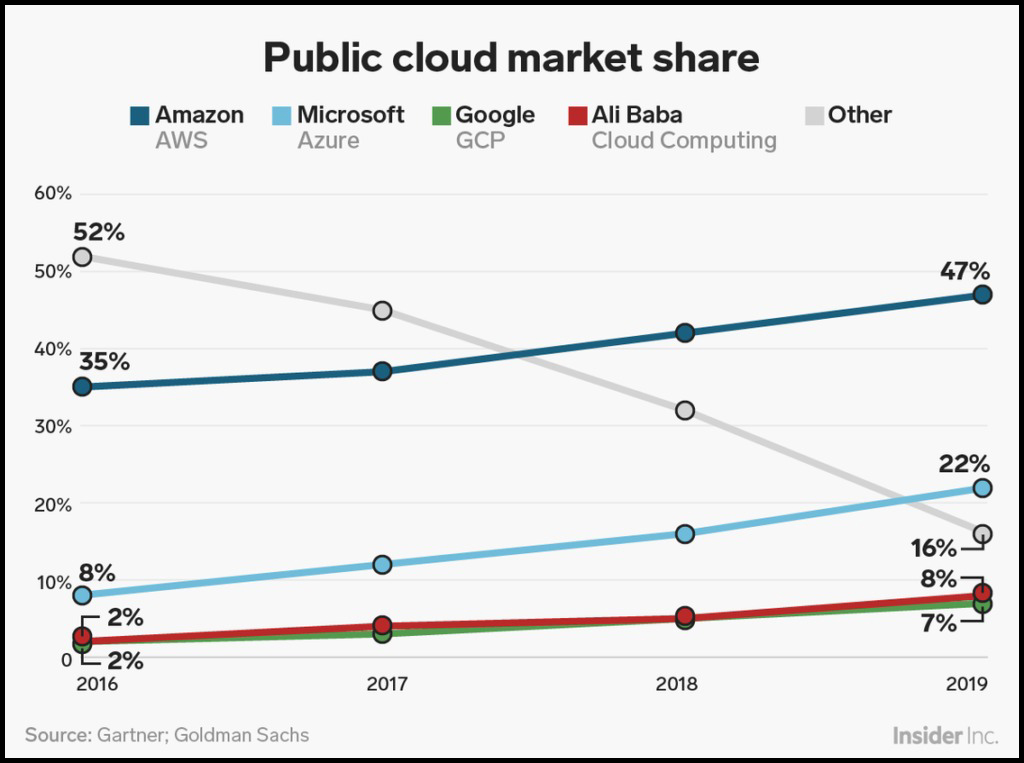
\includegraphics[scale=0.3]{Imagens/awsNomercadoCloud.jpg}
        \fonte{SERVICES(2019a)}
        \label{fig:awsnuvem}
\end{figure}

\subsubsection{Relational Database Service}
Um dos serviços oferecidos pela AWS é o RDS (Serviço de Base de dados relacionais), oferecendo poder de armazenamento sob demanda, evitando que desenvolvedores tenham que lidar com tarefas administrativas, podendo então concentrar-se somente no desenvolvimento. 
Com RDS é possível que o DBA coloque sua base de dados em zonas de disponibilidade, onde se cria o banco de dados em uma destas e habilita a função multi-AZ, fazendo com que o seu banco de dados fique replicado e sincronizado em tempo real, garantindo ainda mais segurança para seus dados e que este nunca pare, mesmo em caso de falha (caso ocorra a base de dados secundária assume exatamente onde a primeira estava).
O RDS da Amazon oferece vários tipos de instâncias de banco de dados, bem como oferece os principais mecanismos de bancos relacionais: SQL Server, Oracle Database, PostgreSQL, MariaDB, MySQL e até mesmo seu próprio mecanismo de banco de dados Amazon Aurora.
\cite{reladataservice}

\subsubsection{Elastic Beanstalk}
Outro serviço oferecido pela AWS é o Elastic Beanstalk, voltado para implantação de aplicações e serviços web desenvolvidos em Kotlin, .NET, PHP, Ruby, Go e Docker, em servidores mais utilizados como Apache, Nginx, Passenger e ISS. 
Assim como o RDS, o Elastic Beanstalk oferece diversas vantagens, como: escalabilidade, extensibilidade, toda a comodidade ao desenvolvedor, abstendo-o das atividades exaustiva de administração/configuração, propiciando que o mesmo só faça o \textit{upload} de seu código e o Elastic Beanstalk se encarregue de todo o gerenciamento da infraestrutura do servidor, como balanceamento de carga, redirecionamento http, conteiners e a execução do servidor propriamente dito, sendo seu maior atrativo o ganho de produtividade.
\cite{elasticbean}


\subsection{Google Cloud Platform}
A definição da própria Google sobre sua plataforma é: “O GCP consiste em um conjunto de ativos físicos, como computadores e unidades de disco rígido, e recursos virtuais, como máquinas virtuais (VMs), localizados nos centros de dados do Google em todo o mundo.” Em outras palavras alugamos parte do armazenamento de um \textit{Data Center} da Google, assim aproveitando uma infraestrutura de alta qualidade e extremamente segura pagando um valor simbólico.
Um fator que diferencia a hospedagem no Google Cloud é a sua rede toda feita com fibra óptica, que faz com que a perca de dados seja quase nula e com taxa de transferência extremamente alta. 
\cite{googlecp}

Segundo o \cite{googlecp} as principais vantagens são:
\begin{itemize}
\item Criação de aplicações de forma rápida;
\item Suportam Linux e Windows;
\item Boa base de conhecimento para solução de problemas.
\end{itemize}

\subsubsection{Application Programming Interface (API)}
API’s (Interface de Programação de Aplicações), são conjuntos de padrões/protocolos que permitem a construção e utilização de aplicativos de forma não tão evidente para usuários, onde sua solução ou serviço pode se comunicar com outros serviços sem precisar saber como eles foram implementados. Possibilitando assim, liberar o acesso aos seus recursos sem abrir mão da segurança e controle. Onde o desenvolvedor é quem define como isso será feito e quem terá acesso.
As API’s surgiram nos primórdios da computação, bem antes dos computadores domésticos, quando eram usadas como bibliotecas de sistemas operacionais.
O foco das API'S é simplificar a integração de novos componentes de aplicações a uma arquitetura já existente.
As API’s públicas acrescentam grande valor comercial porque simplificam e ampliam a forma como você se conecta aos parceiros, além de possivelmente monetizar seus dados. Um exemplo clássico é a API do Google Maps.
\cite{apiredhat}

\subsubsubsection{Routes}
Routes é uma API da Google Cloud voltada para mapas, sua função é disponibilizar o melhor trajeto entre dois pontos, levando em conta fatores como trânsito em tempo real.
É um serviço bastante completo, contendo 64 milhões de estradas catalogadas, 25 milhões de atualizações diárias e 1 bilhão de usuários ativos por mês, segundo informações da própria Google Cloud.
Tudo isso possibilita aos usuários ter o melhor trajeto entre origem e destino, podendo reduzir custos e tempo, seja por transporte coletivo ou privado.
Outro detalhe bastante interessante é o fato de exibir estimativas de trajetos em diversas formas de transportes, como de carro, ônibus/metrô, bicicleta e até mesmo a pé. 
Esta API possui três recursos essenciais:
Directions: Disponibiliza rota de transportes público ou privado, calculando o tempo de deslocamentos atuais ou futuros baseando-se no trânsito em tempo real.
Distance Matrix: Fornece distâncias de um ou mais trajetos e o tempo gasto neste.
Roads: Determina precisamente, o trajeto de um veículo.

As informações obtidas pela API dar-se por meio de interface HTTP, usando coordenadas de latitude e longitude para identificar os locais, acompanhando ainda sua chave de API. A plataforma de mapas do Google é paga, seu valor depende dos recursos integrados a ela, sendo levado em conta também o número de requisições de rotas ou distâncias. Entretanto, disponibilizam de forma gratuita um pacote de recursos com número relativamente alto de requisições, o que atendeu perfeitamente esse projeto.
\cite{routes}


\section{Engenharia de Software}
Embora a “crise do \textit{software}” tenha ocorrido em 1970, parece que esta nunca acaba, pois na atualidade muitos dos problemas enfrentados na época ainda rodeiam desenvolvimento de \textit{softwares}, desde projetos pequenos a sistemas super completos. Os problemas ainda assombram equipes de desenvolvimento, pois muitas das etapas e processos de engenharia de \textit{software} são negligenciados, seja por falta de interesse em produzir um bom \textit{software}, falta de verba para projeto, tempo mal gerenciado e etc.
A engenharia de software nasceu nos primórdios dos anos 70, durante “A crise do software”, onde projetos extrapolavam o prazos e orçamentos, \textit{softwares} possuíam baixíssimas qualidades e diversos problemas. Com o objetivo de saná-los, a engenharia de software surge com ferramentas, técnicas e processos sistematizados de se produzir software, os quais são aplicados nas fases de análise de projeto, documentação, desenvolvimento, validação, implantação, e evolução de software.
Dentre os diversos problemas que ainda persistem até então, pode se destacar:
Levantamento de requisitos mal feitos, onde equipes com a falsa sensação de produtividade já querem codificar de forma imediata, e para tal não absorvem as necessidades do cliente. Por outro lado, clientes omitem informações que, embora para ele seja óbvia mas para a equipe de desenvolvimento não.
Falta de comunicação entre cliente e desenvolvedor, esse problema ocorre dos dois pontos de vista, da visão de cliente, pensam que a equipe conhece totalmente suas necessidades, e muitos detalhes não são passados. Por outro lado, a equipe de desenvolvimento pode não ser muito detalhista quanto ao que é possível de se solucionar com softwares por exemplo.
Diversas organizações contratam gerentes de projetos com pouco \textit{know-how} ou ainda sem nenhum conhecimento de tecnologia. Estes muitas vezes possuem a falsa sensação de que ter equipamentos de modernos é o suficiente para sua equipe alcançar um \textit{software} de sucesso, ou ainda contratar mais programadores é a solução para o cronograma estourado.
Muitas empresas negligenciam por exemplo, a documentação de software, e no caso de contratação de nova equipe de desenvolvimento, torna se árduo sua manutenibilidade, já que a equipe não terá nenhuma base para conhecer o projeto. Fases de manutenção são ainda mais custosas que o desenvolvimento em si. \textit{Softwares} devem ser criados visando fácil manutenibilidade, atender requisitos de clientes, ter um bom padrão de qualidade, ser confiável e etc., pois o sucesso de uma empresa de desenvolvimento depende disso.
Para tal, técnicas de engenharia de software devem ser bem empregadas do início ao fim do projeto, ou ainda por toda sua existência, visando ter total controle do projeto. É possível que no futuro, as próprias tecnologias substituam programadores, mas nunca substituirá técnicas de engenharia de software.
\cite{engenhariadesoftware}


\section{Front-End}
O front-end é o cartão de visitas para uma aplicação, pois é neste que o usuário tem sua primeira impressão, antes mesmo de usá-la. Esta camada é crucial na comunicação/marketing da empresa pois no design deste, utiliza-se geralmente logotipos da empresa ou pelo menos padrões de cores relacionados a essa. Um front-end bem elaborado irá despertar nos usuários da aplicação, uma confiança de um software bem desenvolvido, e até mesmo definir o sucesso ou fracasso da aplicação.
\cite{universoprograma}

\subsection{Flutter}
Com a mesma proposta do React Native de criar aplicativos híbridos utilizando apenas uma base de código surgiu o Flutter em 2017, desenvolvido e atualizado pela equipe da Google, utilizando a linguagem Dart como base de criação dos aplicativos.
O Flutter fica na camada do UI e não chama os componentes nativos do SO, diferente do React Native que possui um intermediário entre a UI e o dispositivo. Trabalhando dessa forma traz uma performance muito mais rápida e fluida, e pode até mesmo ser comparada a um aplicativo feito de maneira nativa. Sua curva de aprendizado também é muito rápida e simples.
O Flutter trabalha com os "\textit{widgets}", que seria a mesma coisa de um componente. Um \textit{widget} é uma árvore que pode conter um ou mais filhos, e esses filhos são renderizados conforme a construção desta árvore. 
\cite{flutter}
A figura a seguir demonstra

\begin{figure}[H]
    \centering
        \caption{Um gráfico de radar mostrando a nota de 0–5 para cada critério em cada plataforma.}
        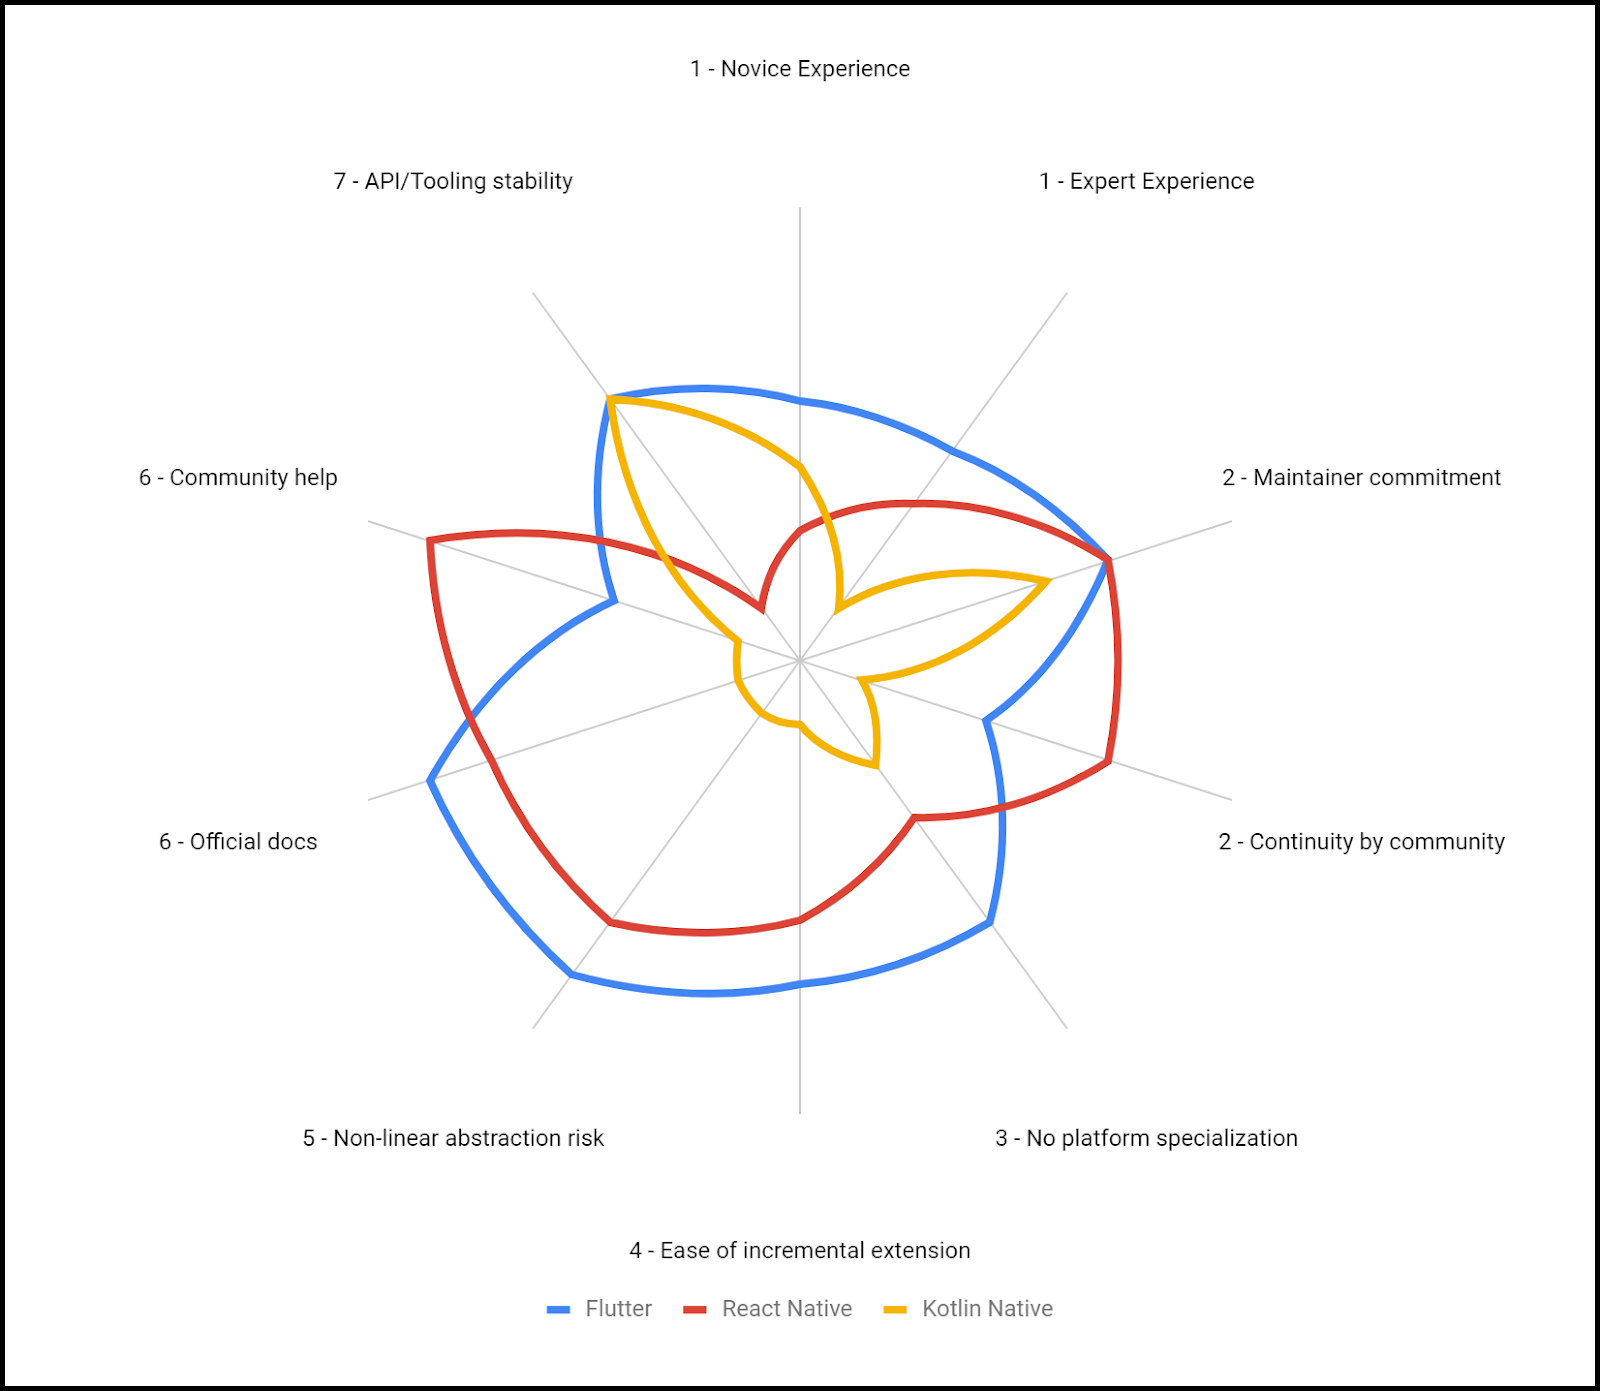
\includegraphics[scale=0.3]{Imagens/flutter.png}
        \fonte{(FREIRE,2019)}
        \label{fig:flutter}
\end{figure}


\section{Plataforma Mobile}
É indiscutível o uso de \textit{smartphone} atualmente, pois só no Brasil tem mais de um aparelho por pessoa, segundo a 29ª Pesquisa Anual de Administração e Uso de Tecnologia da Informação nas Empresas, realizada pela Fundação Getúlio Vargas de São Paulo (FGV-SP).

Sabendo disso, é notável a importância de se desenvolver para essa plataforma, além de outros fatores os quais aplicações \textit{mobile} se sobressaem entre as demais. Por exemplo, em uma aplicação \textit{web} tem se um tempo bem superior ao se conectar com um servidor, se comparado a um aplicativo mobile.
\cite{meirellespesquisa29}


%%%%%%%%%%%%%%%%%%%%%%%%%%%%%%%%%%%%%%%%%%%%%%%%%%%%%
%% Inserir seu texto da metodologia no campo abaixo %%
%%%%%%%%%%%%%%%%%%%%%%%%%%%%%%%%%%%%%%%%%%%%%%%%%%%%%
\chapter{Metodologia} 

\section{Tipo de Pesquisa}
O tipo de pesquisa escolhida foi quantitativa e exploratória, visando a viabilidade em se  desenvolver um aplicativo para busca de menor preço para uma compra com rota otimizada. O levantamento bibliográfico constitui-se de material já publicado de artigos científicos, livros, revistas e sites renomados da área.

\section{Método de Realização}
A opção pela pesquisa quantitativa tem por objetivo analisar o ponto de vista do público alvo do aplicativo proposto visando sua aceitação e viabilidade, podendo assim saber se uma aplicação de suporte a compras domésticas que tem por intuito oferecer a seus usuários onde encontrar o menor preço para suas compras levando em conta a melhor rota para tal é algo que a sociedade realmente precisa.

\section{Coleta de Dados}
Os dados foram levantados através de um formulário o qual foi disponibilizado de forma online para um grupo de 53 pessoas. Tais informações adquiridas com este foram essenciais para validar a viabilidade do projeto. 

Veja a seguir os dados levantados com tal formulário, no qual um grupo considerável de pessoas participaram:

Como esperado, mais de 75\% dessa população vai aos supermercados 2 a 10 vezes ao mês, conforme pode ser visto na figura \ref{fig:metodologia1}:

\begin{figure}[H]
    \centering
        \caption{Pergunta 01}
        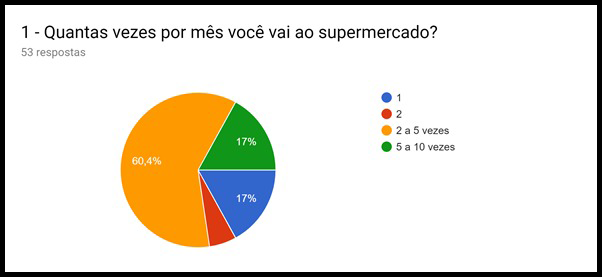
\includegraphics[scale=.8]{metodologia1.png}
        \label{fig:metodologia1}
		\fonte{Do autor - 2019}
\end{figure}


A maioria das pessoas sempre visita mais de um estabelecimento a fim de encontrar aquele que ofereça o melhor preço, conforme pode ser visto na figura \ref{fig:metodologia2} abaixo:

\begin{figure}[H]
    \centering
		\caption{Pergunta 02}
		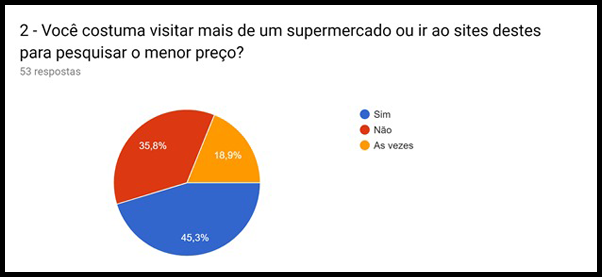
\includegraphics[scale=.8]{metodologia2.png}
		\label{fig:metodologia2}
		\fonte{Do autor - 2019}
\end{figure}

Nas visitas realizadas para a pesquisa de preço, há obviamente os gastos com transportes, seja de automóvel próprio ou transporte coletivo. A figura \ref{fig:metodologia3} traz esta informação.

\begin{figure}[H]
    \centering
		\caption{Pergunta 03}
		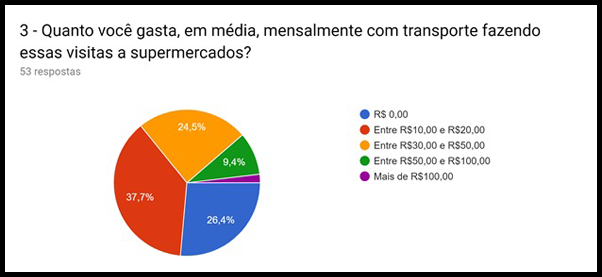
\includegraphics[scale=.8]{metodologia3.png}
		\label{fig:metodologia3}
		\fonte{Do autor - 2019}
\end{figure}

Há um gasto de tempo consideravelmente alto, levando em conta que para uma compra pessoas gastem tanto tempo visitando os supermercados. Demonstrado figura \ref{fig:metodologia4} abaixo.

\begin{figure}[H]
    \centering
		\caption{Pergunta 04}
		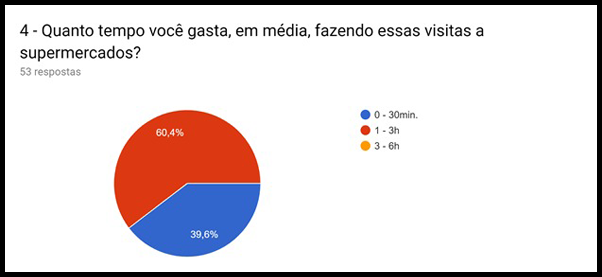
\includegraphics[scale=.8]{metodologia4.png}
		\label{fig:metodologia4}
		\fonte{Do autor - 2019}
\end{figure}

Indiscutivelmente, todas as pessoas entrevistadas usariam o aplicativo proposto. Conforme pode ser visto na figura \ref{fig:metodologia5}:
\begin{figure}[H]
    \centering
		\caption{Pergunta 05}
		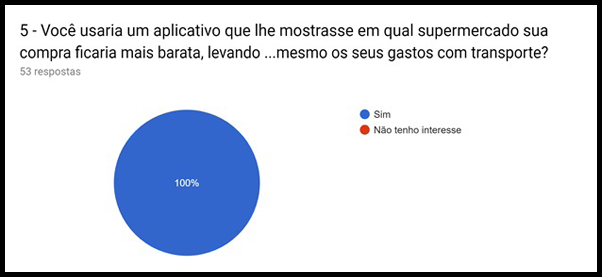
\includegraphics[scale=.8]{metodologia5.png}
		\label{fig:metodologia5}
		\fonte{Do autor - 2019}
\end{figure}

Pode se notar ainda que, quando se trata do tão escasso tempo, as pessoas estão dispostas a  abrirem mão da tão tradicional “experiência de compra”. O que pode ser visto na figura \ref{fig:metodologia6}.

\begin{figure}[H]
    \centering
		\caption{Pergunta 06}
		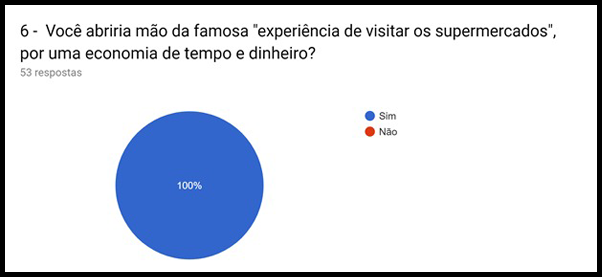
\includegraphics[scale=.8]{metodologia6.png}
		\label{fig:metodologia6}
		\fonte{Do autor - 2019}
\end{figure}

O formulário continha ainda questão aberta, visando analisar de forma mais dinâmica as opiniões dos supostos usuários: "... Um aplicativo que disponibiliza a seus usuários os menores preços para seus produtos, evitando que este, tenha gasto desnecessário de tempo e dinheiro fazendo pesquisas de preço..."
Na sua opinião, um supermercado aderiria um aplicativo com tal finalidade?

Foram obtidas diversas opiniões, as quais proporcionaram pontos de vista até então não trabalhados, porém prevaleceram as opiniões de pessoas que afirmaram ser totalmente necessário o uso do aplicativo na sociedade. Dentre as mais relevantes, pode se destacar:
“Sim, pois facilitaria imensamente a vida dos clientes dos supermercados, e os comércios devem adaptar-se aos clientes e não o contrário.”
“Sim, por saber que outros ramos do comércio já utilizam ferramentas do tipo para facilitar o alcance ao cliente. ”

Foi questionado também se as pessoas estariam dispostas a pagarem pelo uso do aplicativo, e pelo menos cerca de 1/3 destes se negaram a pagar, tal perspectiva reforça a hipótese de passar o custo diretamente para o estabelecimento ao invés de clientes ou cobrando 8\% encima de toda venda feita com o auxílio do aplicativo.

Um outro fato que ao ser inserido no aplicativo, e que poderia beneficiar tanto os estabelecimentos (divulgação de promoções) quanto clientes. Como é demonstrado na figura \ref{fig:metodologia9}.

\begin{figure}[H]
    \centering
		\caption{Pergunta 09}
		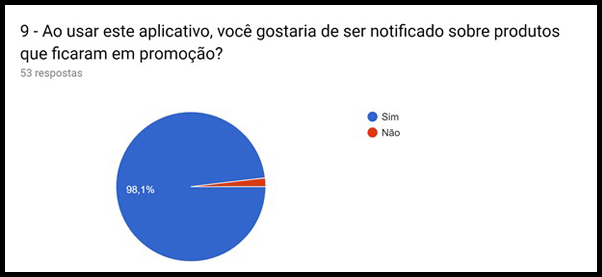
\includegraphics[scale=.8]{metodologia9.png}
		\label{fig:metodologia9}
		\fonte{Do autor - 2019}
\end{figure}

% \section{Critérios de Delimitação}
% Digite seu texto nesse campo.

% \section{Instrumentos de Pesquisa}
% Digite seu texto nesse campo.

% \section{Tratamento dos Dados}
% Digite seu texto nesse campo.

\chapter{Desenvolvimento}

\section{Diagrama de casos de uso}
\begin{figure}[H]
	\centering
		\caption{Diagrama de casos de uso.}
		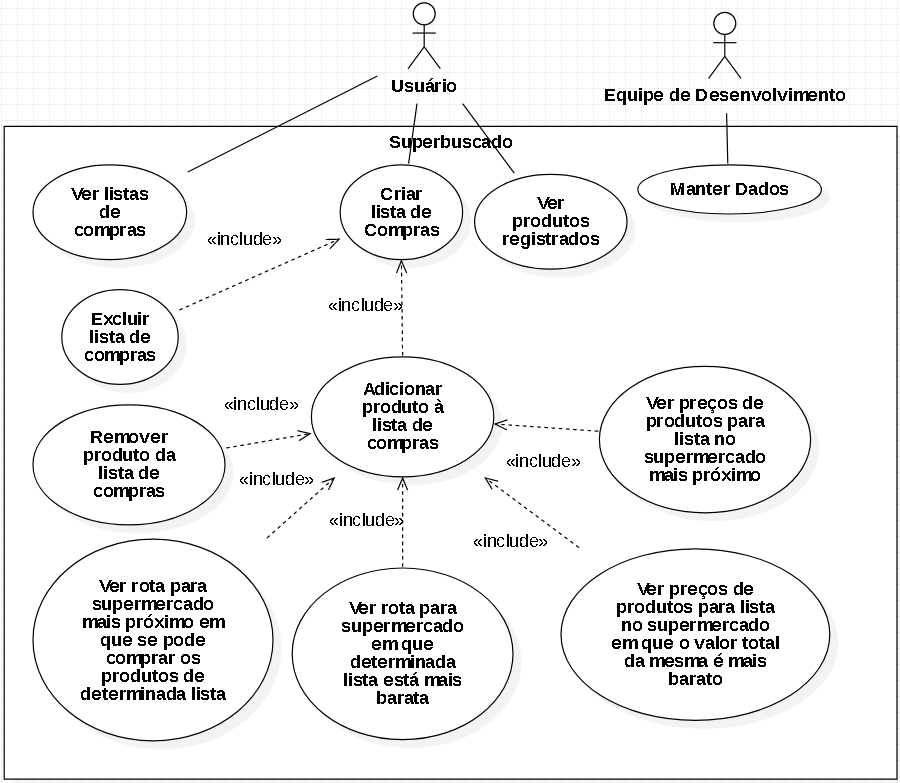
\includegraphics[scale=0.4]{Imagens/DiagramaDeCasosDeUso.png}
		\fonte{Do autor - 2019.}	
\end{figure}


\section{Especificações de caso de uso}
As  atividades que podem ser realizadas no aplicativo e os atores participantes destas, estão descritas nas sequências de imagens abaixo, figura  \ref{fig:UC001} até \ref{fig:UC010}.
\begin{figure}[H]
    \centering
        \caption{UC001.}
        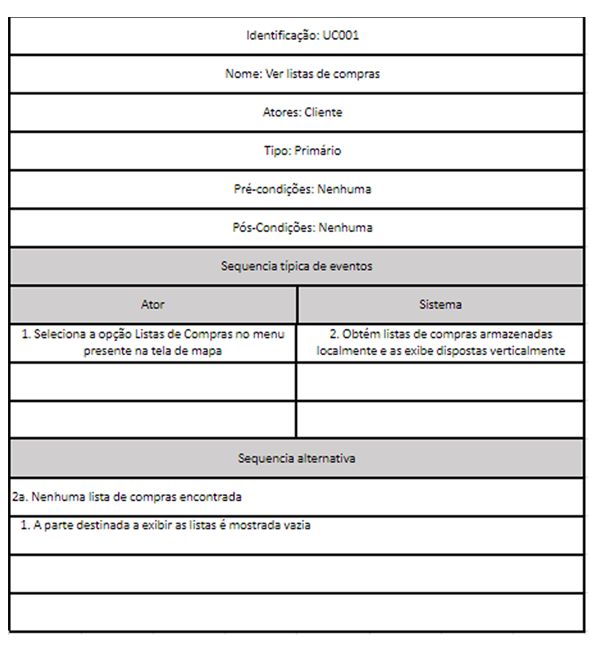
\includegraphics[scale=0.8]{Imagens/UC001.PNG}
        \fonte{Do autor - 2019.}
        \label{fig:UC001}
\end{figure}
	
\begin{figure}[H]
	\centering
		\caption{UC002}
		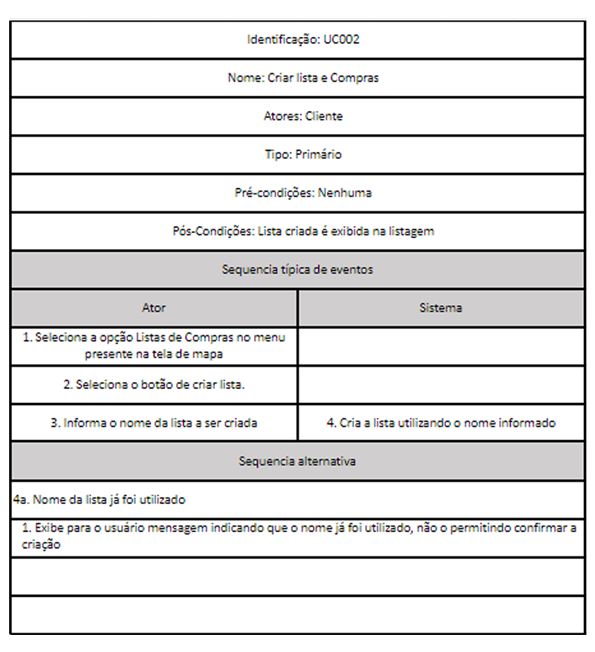
\includegraphics[scale=0.8]{Imagens/UC002.PNG}
		\fonte{Do autor - 2019.}
\end{figure}
	
\begin{figure}[H]
	\centering
		\caption{UC003}
		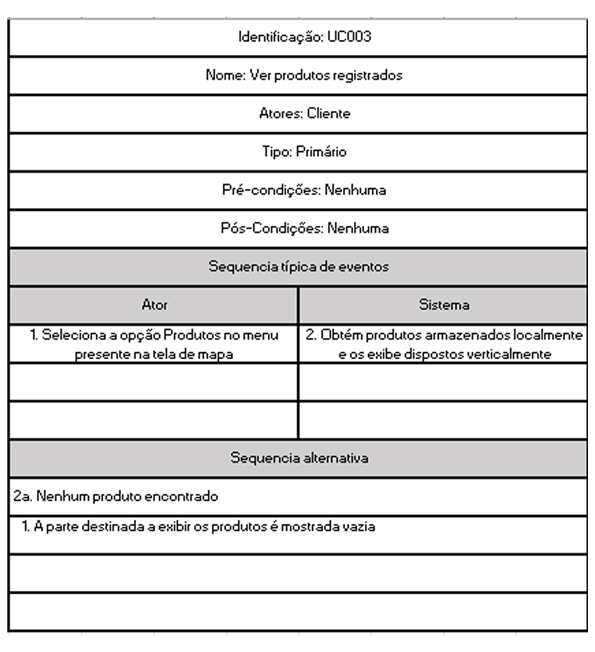
\includegraphics[scale=0.8]{Imagens/UC003.PNG}
		\fonte{Do autor - 2019.}
\end{figure}

\begin{figure}[H]
	\centering
		\caption{UC004}
		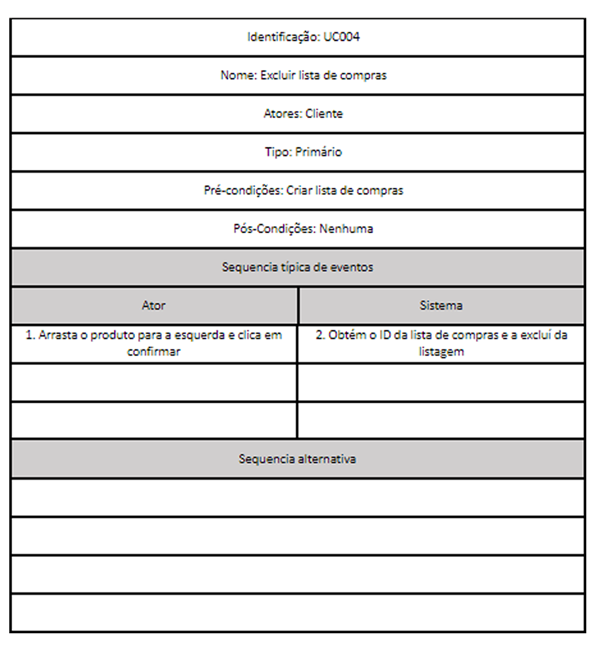
\includegraphics[scale=0.8]{Imagens/UC004.PNG}
		\fonte{Do autor - 2019.}
\end{figure}
	
\begin{figure}[H]
	\centering
		\caption{UC005}
		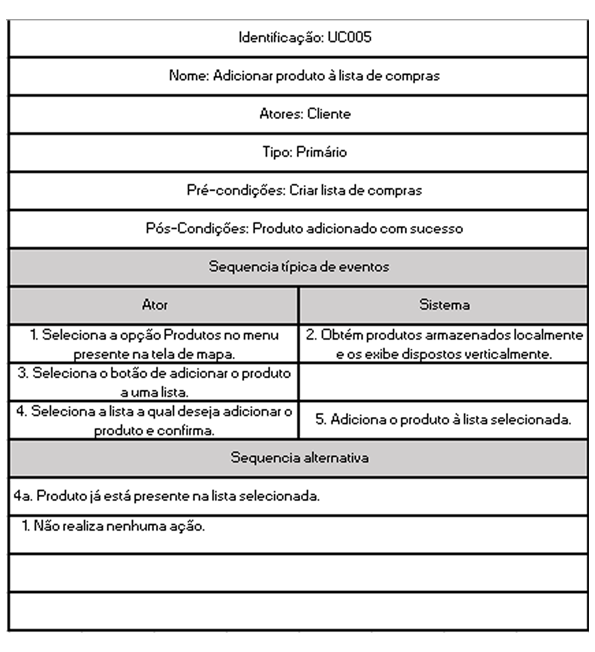
\includegraphics[scale=0.8]{Imagens/UC005.PNG}
		\fonte{Do autor - 2019.}
\end{figure}

\begin{figure}[H]
	\centering
		\caption{UC006}
		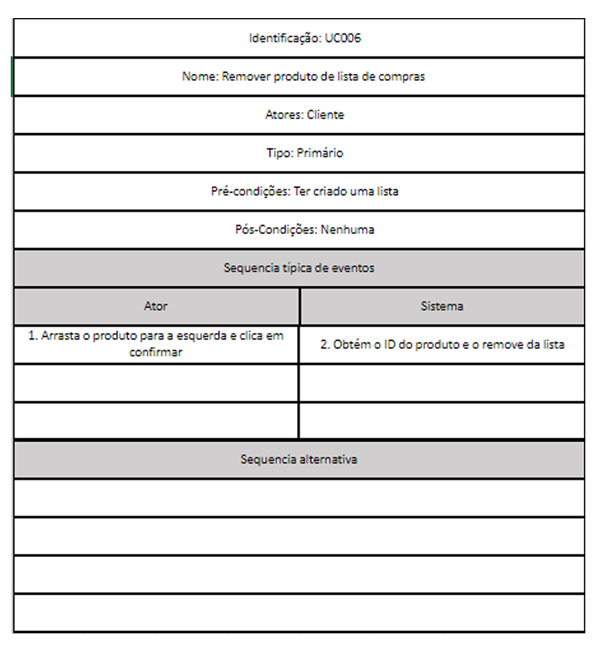
\includegraphics[scale=0.8]{Imagens/UC006.PNG}
		\fonte{Do autor - 2019.}
\end{figure}

\begin{figure}[H]
	\centering
		\caption{UC007}
		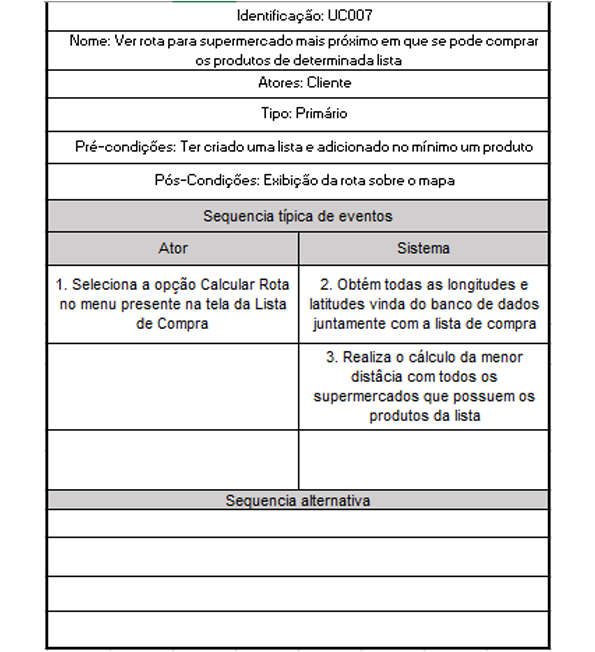
\includegraphics[scale=0.8]{Imagens/UC007.PNG}
		\fonte{Do autor - 2019.}
\end{figure}
	
\begin{figure}[H]
	\centering
		\caption{UC008}
		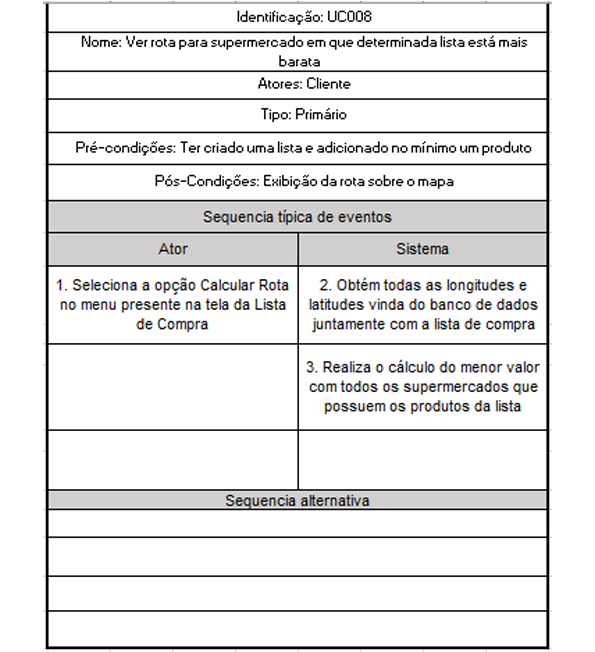
\includegraphics[scale=0.8]{Imagens/UC008.PNG}
		\fonte{Do autor - 2019.}
\end{figure}
	
\begin{figure}[H]
	\centering
		\caption{UC009}
		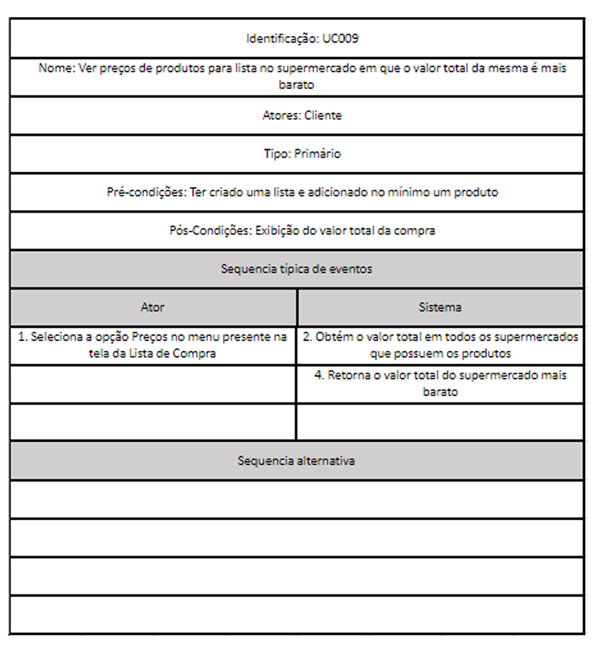
\includegraphics[scale=0.8]{Imagens/UC009.PNG}
		\fonte{Do autor - 2019.}
\end{figure}
	
\begin{figure}[H]
	\centering
		\caption{UC010}
		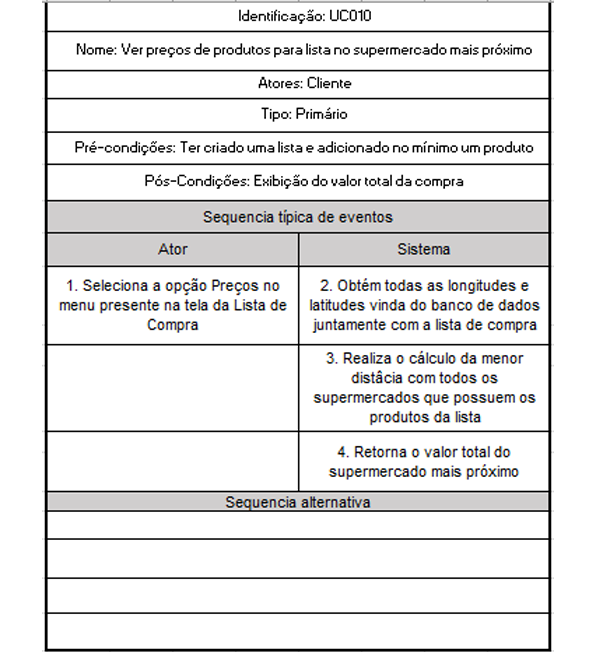
\includegraphics[scale=0.8]{Imagens/UC010.PNG}
		\fonte{Do autor - 2019.}
		\label{fig:UC010}	
\end{figure}


\section{Diagrama de atividades}
	Faz-se necessário descrever o algoritmo de forma bem explícita, e para tal, foi utilizado um diagrama de atividades, como vemos na figura \ref{fig:fluxograma}, o qual descreve sequência operacional das ações e tomadas de decisões que o usuário pode realizar no aplicativo.
	
\begin{figure}[H]
	\centering
		\caption{Diagrama de atividades do aplicativo Superbuscado}
		\includegraphics[scale=0.3]{Imagens/fluxograma.PNG}
		\fonte{Do autor - 2019.}
		\label{fig:fluxograma}	
\end{figure}

\section{Análise de requisitos}
\begin{itemize}
\item [RF001] O usuário deve ser capaz de visualizar no mapa os supermercados identificados com um marcador.
\item [RF002] O usuário deve ser capaz ver a lista dos produtos cadastrados, cada qual com nome, foto, categorias e preços, além de poder pesquisa-los pelo nome.
\item [RF003] O usuário deve ser capaz de criar e apagar listas de compras.
\item [RF004] O usuário deve ser capaz de adicionar e remover produtos de listas de compras.
\item [RF005] O usuário deve ser capaz de visualizar todos os produtos contidos em uma determinada lista de compras.
\item [RF006] O usuário deve ser capaz de visualizar a lista de compras feita tanto no supermercado em que ela se encontra mais barata quanto naquele em que a distância de deslocamento até o estabelecimento for menor.
\item [RF007] O usuário deve ser capaz de ver tanto a rota para o supermercado em que determinada lista de compras possui seu menor preço quanto para a rota direcionada para o supermercado com menor distância de deslocamento.
\end{itemize}

\begin{itemize}
\item [RNF001] O aplicativo não deve permitir a utilização com o GPS desligado.
\item [RNF002] O aplicativo deve manter suas telas atualizadas quando ocorrerem mudanças nos dados.
\item [RNF003] O aplicativo não deve sobrepor a menor rota no mapa com a rota mais barata.
\end{itemize}


\section{Análise de dados}
Para testar o desempenho do aplicativo, foram realizadas diversas possibilidades com rotas e quantidades de produtos, os resultados obtidos podem ser analisados na figura \ref{fig:tabelaestado}. Para tal teste, foram utilizados um Motorola Moto One Zoom (Processador: 8 core 1.8 GHZ, 3GB de RAM) e Xiaomi Redmi Note 7 (Processador: 8 core 2.0 GHZ, 3GB de RAM).

\begin{figure}[H]
   	\centering
   		\caption{Testes nos celulares Motorola Moto One Zoom e Xiaomi Redmi Note 7.}
	   	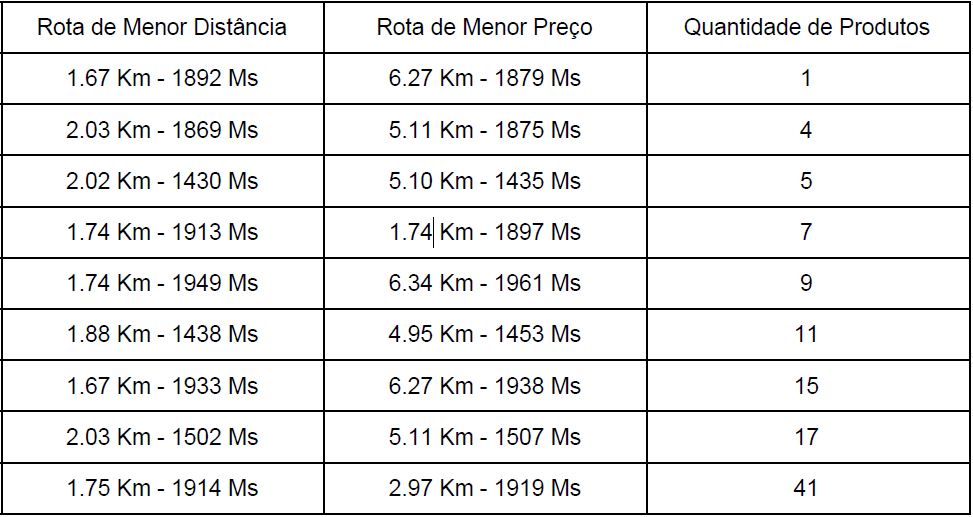
\includegraphics[scale=0.64]{Imagens/AnaliseDeDados.PNG}
   		\fonte{Do autor - 2019}
   		\label{fig:tabelaestado}
\end{figure}

Após uma análise profunda da performance no procedimento de cálculo de rota, notamos que o
tempo de execução é basicamente o mesmo independente da distância e do número de
produtos. Foi constatado também que a média do tempo de execução dos cálculos da menor
rota e da rota mais barata foram executados com tempos médios semelhantes. Baseando-se
nesses fatos, pode-se concluir que a complexidade de tempo de ambos pode ser considerada
a mesma levando em conta uma pequena margem de erro.

\begin{itemize}
\item Nos testes a média aritmética da menor distância foi de 1760 Ms.
\item Nos testes a média aritmética do menor preço foi de 1763 Ms.
\end{itemize}


\section{Documentação do banco de dados}
\subsection{Requisitos e regras de negócio}

\subsection{Estado}
	Entidade de unidades federativas, as quais fazem parte do endereço de um supermercado, o nome de estado é obrigatório e nunca irá se repetir, já que não existe mais de um estado com mesmo nome em um país.
	
\subsection{Cidade}
	Entidade cidades dos supermercados, várias cidades podem pertencer a um estado, mas uma cidade só pertence a um estado ao mesmo tempo, um nome de cidade pode existir em outro estado (nesse caso, cada cidade será tratada de forma diferente, de forma exclusiva), mas nunca poderá existir mais de uma cidade com mesmo nome em um único estado. Cada cidade deve obrigatoriamente ter um nome e estado.

\subsection{Bairro}
	Entidade de bairro dos supermercados, uma cidade pode ter vários bairros, mas um bairro só pode pertencer a uma cidade ao mesmo tempo, não pode haver bairros com mesmo nome em uma cidade, mas em outra cidade poderá ser aceito (nesse caso, cada bairro será tratado de forma diferente, como único). Todo bairro deverá ter nome, e uma cidade a ele relacionada, bem como uma cidade tem um estado. 

\subsection{Supermercado}
	Supermercado deve ter um bairro, que por sua vez deve ter uma cidade e essa ter um estado. Em um bairro pode haver diversos supermercados. Pode haver repetições de nomes de supermercados, porém cada um destes será tratado de forma diferente, como único. Cada supermercado deverá ter obrigatoriamente um nome, logradouro, bairro, latitude, longitude, opcionalmente pode ter um site.

\subsection{Produto}
	Cada produto deve ter nome único, não se pode repetir o nome deste, o produto deve pertencer a uma categoria ou mais de uma ao mesmo tempo, este pode estar em diversos supermercados ou em nenhum, ao passo que um supermercado pode ter diversos produtos. 

\subsection{Categoria}
	Uma categoria pode ter diversos produtos ou nenhum, não é permitido existir mais de uma categoria com mesmo nome.
	
\section{Dicionário de dados}
	Um dicionário de dados é fundamental em uma modelagem de banco de dados, sendo este utilizado para armazenar informações sobre o conteúdo, formato e estrutura de um banco de dados. Pode-se dizer que, um dicionário de dados são metadados, já que são dados de outros dados. Tendo em vista o grande potencial deste em uma documentação, segue abaixo (nas figuras \ref{fig:tabelaestado} a \ref{fig:tabelacamposunicos}) o dicionário de dados que tem como objetivo documentar o banco de dados usado no aplicativo.
	
\begin{figure}[H]
	\centering
	\caption{Tabela Estado.}
	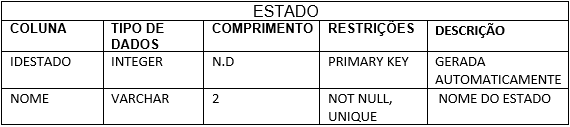
\includegraphics[scale=0.64]{Imagens/TabelaEstado.PNG}
	\fonte{Do autor - 2019}
    \label{fig:tabelaestado}
\end{figure}
						
\begin{figure}[H]
	\centering
    \caption{Tabela Cidade.}
    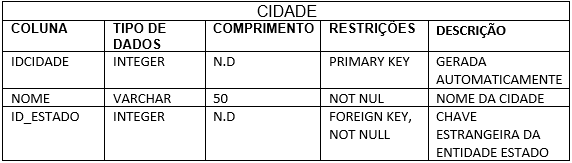
\includegraphics[scale=0.64]{Imagens/TabelaCidade.PNG}
    \fonte{Do autor - 2019}
\end{figure}
			
\begin{figure}[H]
    \centering
    \caption{Tabela Bairro.}
   	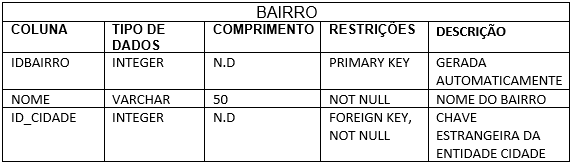
\includegraphics[scale=0.64]{Imagens/TabelaBairro.PNG}
  	\fonte{Do autor - 2019}
\end{figure}
			
\begin{figure}[H]
	\centering
    \caption{Tabela Supermercado.}
    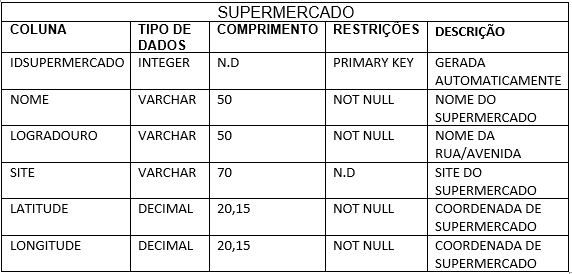
\includegraphics[scale=0.64]{Imagens/TabelaSupermercado.PNG}
    \fonte{Do autor - 2019}
\end{figure}
			
\begin{figure}[H]
    \centering
    \caption{Tabela Supermercado-Bairro.}
    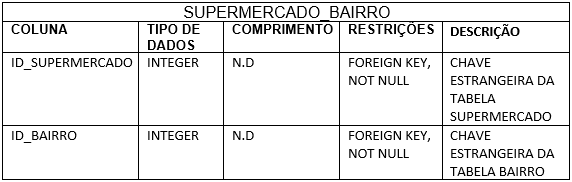
\includegraphics[scale=0.64]{Imagens/TabelaSupermercadoBairro.PNG}
    \fonte{Do autor - 2019}
\end{figure}
			
\begin{figure}[H]
    \centering
    \caption{Tabela Produto.}
    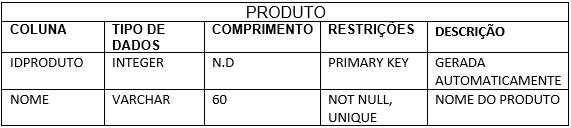
\includegraphics[scale=0.64]{Imagens/TabelaProduto.PNG}
    \fonte{Do autor - 2019}
\end{figure}
			
\begin{figure}[H]
    \centering
    \caption{Tabela Categoria.}
    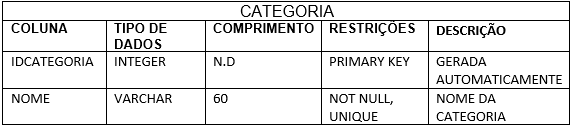
\includegraphics[scale=0.64]{Imagens/TabelaCategoria.PNG}
    \fonte{Do autor - 2019}
\end{figure}
			
\begin{figure}[H]
	\centering
	\caption{Tabela Produto-Categoria.}
	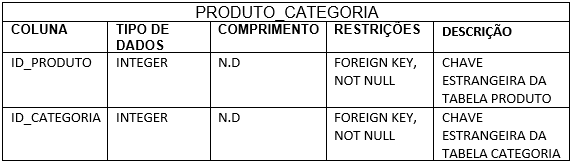
\includegraphics[scale=0.64]{Imagens/TabelaProdutoCategoria.PNG}
	\fonte{Do autor - 2019}
\end{figure}
			
\begin{figure}[H]
	\centering
    \caption{Tabela Supermercado-Produto.}
    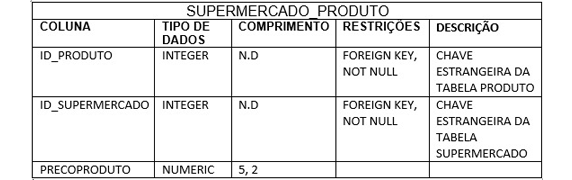
\includegraphics[scale=0.64]{Imagens/TabelaSupermercadoProduto.PNG}
    \fonte{Do autor - 2019}
\end{figure}
			
\begin{figure}[H]
	\centering
   	\caption{Tabela Chaves primárias.}
   	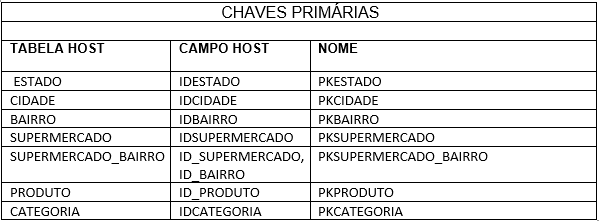
\includegraphics[scale=0.64]{Imagens/TabelaChavesPrimarias.PNG}
   	\fonte{Do autor - 2019}
\end{figure}
			
\begin{figure}[H]
  	\centering
   	\caption{Tabela Chaves estrangeiras.}
   	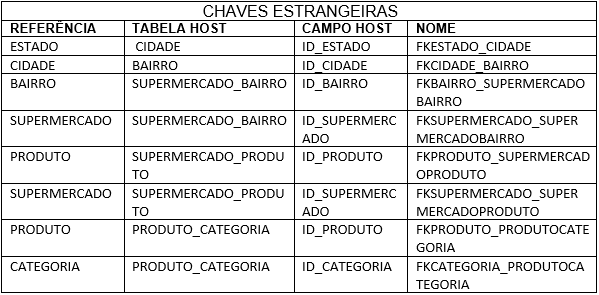
\includegraphics[scale=0.64]{Imagens/TabelaChavesEstrangeiras.PNG}
   	\fonte{Do autor - 2019}
\end{figure}
			
\begin{figure}[H]
  	\centering
   	\caption{Tabela Campos únicos.}
   	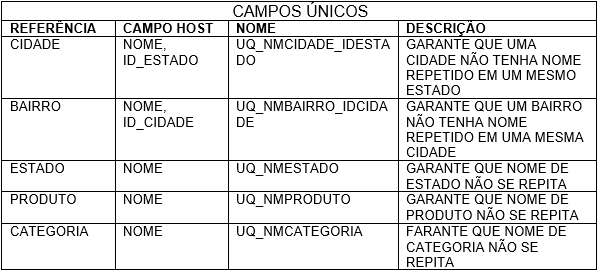
\includegraphics[scale=0.64]{Imagens/TabelaCamposUnicos.PNG}
   	\fonte{Do autor - 2019.}
   	\label{fig:tabelacamposunicos}
\end{figure}
		

\section{Modelagem lógica}
	A modelagem lógica possui o detalhamento da base de dados, de forma que o usuário possa entender facilmente toda a proposta do projeto. É um nível independente de SGBD, seu objetivo visa detalhar o banco de dados tanto para desenvolvedores de banco de dados quanto para os não desenvolvedores. Estão descritas na figura \ref{fig:modelagemlogica} tais representações.
	
\begin{figure}[H]
   	\centering
   	\caption{Modelagem Lógica.}
   	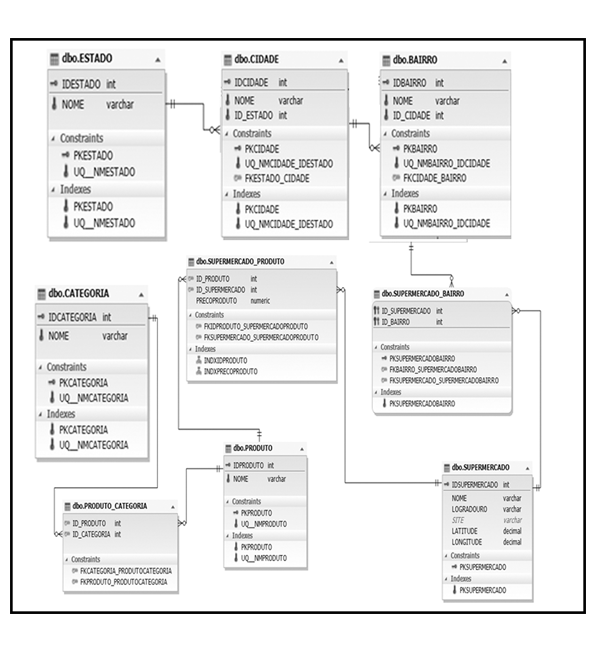
\includegraphics[scale=0.8]{Imagens/ModelagemLogica.png}
   	\fonte{Do autor - 2019.}
   	\label{fig:modelagemlogica}
\end{figure}
	
\section{Modelagem física}
	A modelagem física é o último passo na criação de um banco de dados, tal nível de modelagem depende do SGBD, tendo esses suas peculiaridades e algumas diferenças entre si. Este é o nível mais próximo entre homem e máquina no que se refere a banco de dados, não tem como objetivo detalhar o projeto para usuários, são de fato, scripts para serem processados por máquina, como nas figuras \ref{fig:modelagemfisica01} a \ref{fig:modelagemfisica03}.
	
\begin{figure}[H]
	\centering
	\caption{Modelagem Física - Imagem 01.}
	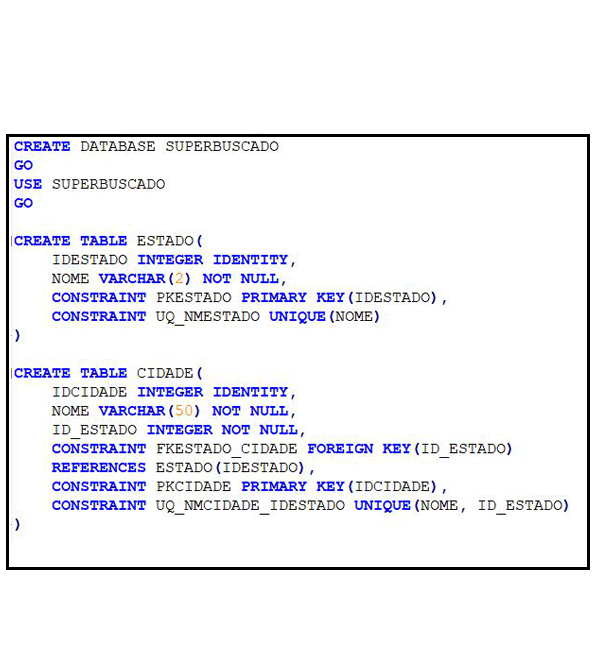
\includegraphics[scale=0.8]{Imagens/ModelagemFisica01.png}
	\fonte{Do autor - 2019.}
	\label{fig:modelagemfisica01}
\end{figure}
			
\begin{figure}[H]
	\centering
    \caption{Modelagem Física - Imagem 02.}
    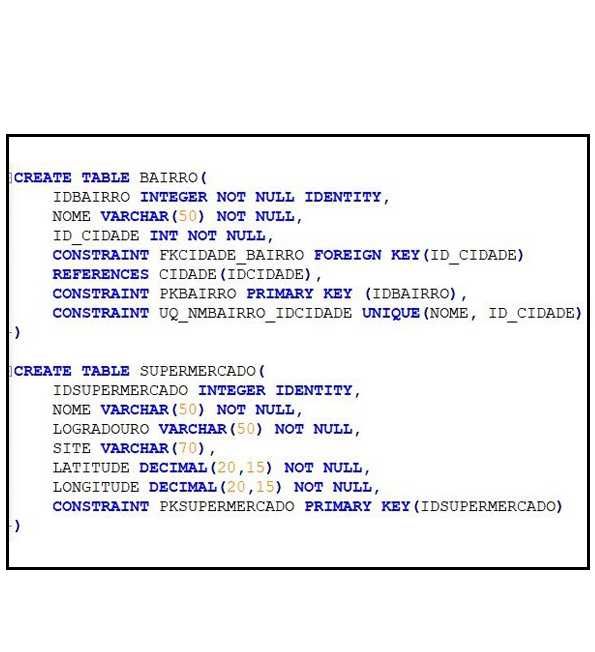
\includegraphics[scale=0.8]{Imagens/ModelagemFisica02.png}
    \fonte{Do autor - 2019.}
    \label{fig:modelagemfisica02}
\end{figure}
			
\begin{figure}[H]
   	\centering
    \caption{Modelagem Física - Imagem 03.}
    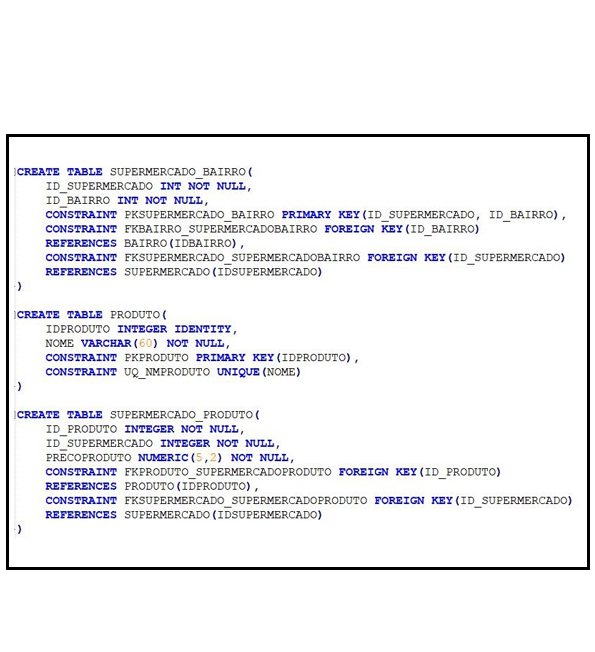
\includegraphics[scale=0.8]{Imagens/ModelagemFisica03.png}
    \fonte{Do autor - 2019.}
\end{figure}

\begin{figure}[H]
   	\centering
    \caption{Modelagem Física - Imagem 04.}
    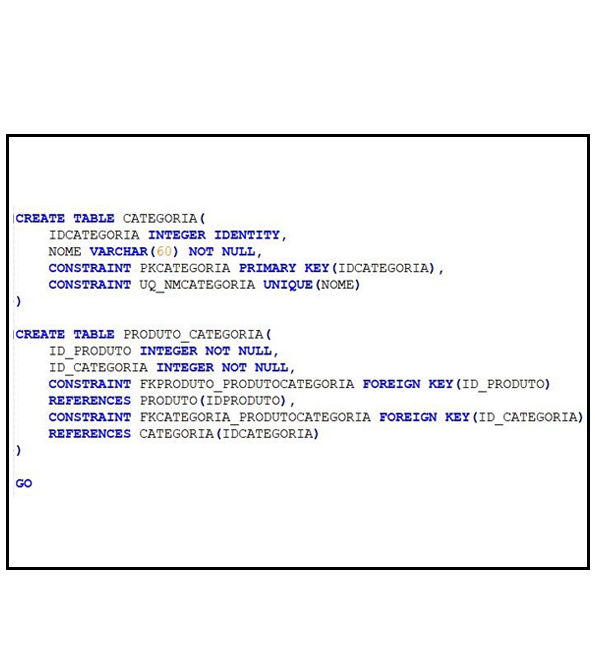
\includegraphics[scale=0.8]{Imagens/ModelagemFisica04.png}
    \fonte{Do autor - 2019.}
\end{figure}

			
\section{Criação de Views}
\begin{figure}[H]
    \centering
    \caption{Criação de Views - Imagem 01.}
    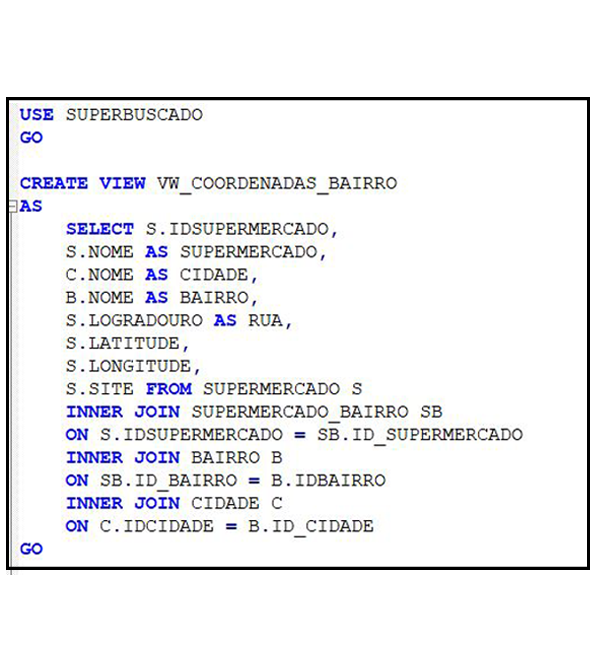
\includegraphics[scale=0.8]{Imagens/CriacaoDeViews01.png}
    \fonte{Do autor - 2019.}
\end{figure}

\begin{figure}[H]
	\centering
   	\caption{Criação de Views - Imagem 02.}
   	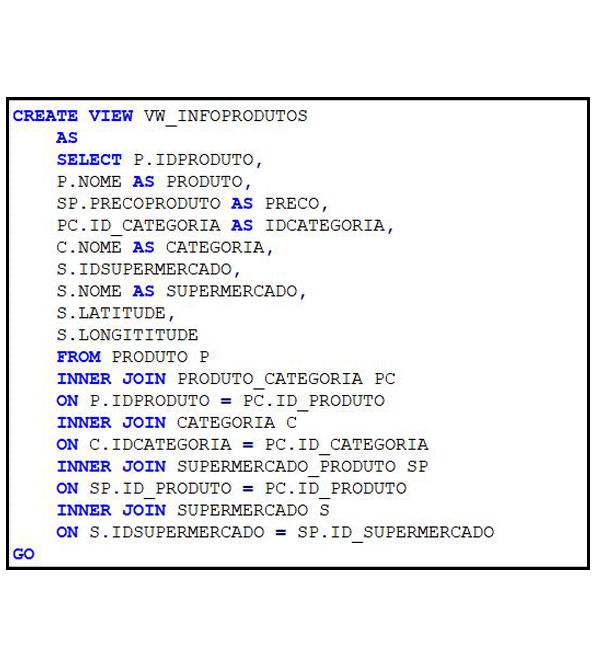
\includegraphics[scale=0.8]{Imagens/CriacaoDeViews02.png}
   	\fonte{Do autor - 2019.}
   	\label{fig:modelagemfisica03}
\end{figure}
			
\subsection{Diagrama de visões}
	\begin{figure}[H]
    \centering
    \caption{Diagrama.}
    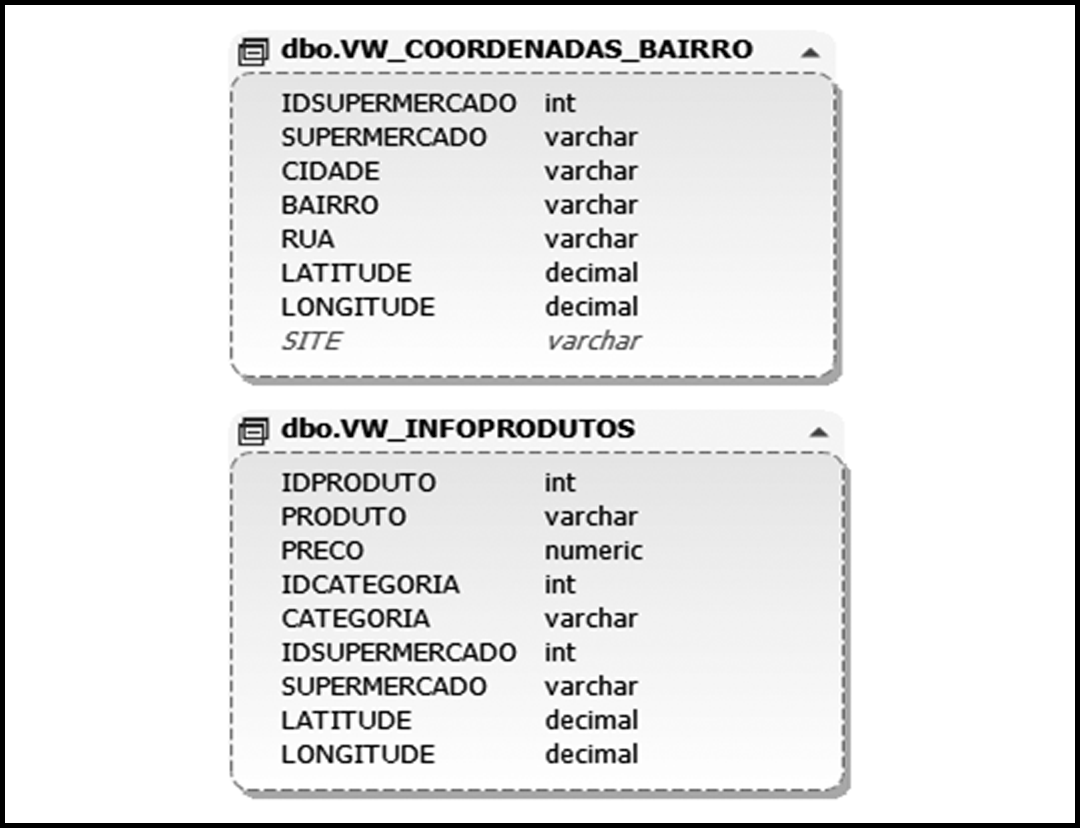
\includegraphics[scale=0.3]{Imagens/ViewsDiagrama.png}
    \fonte{Do autor - 2019.}
\end{figure}

\section{Interface do aplicativo}
Está é a tela inicial da aplicação, começa na área do GPS para garantir que logo no começo do uso todos os itens necessários estejam ativos, além de ser uma funcionalidade a mais, pois assim o usuário pode apenas consultar um caminho para um supermercado específico caso o queira.
\begin{figure}[H]
    \centering
    \caption{Tela Inicial.}
    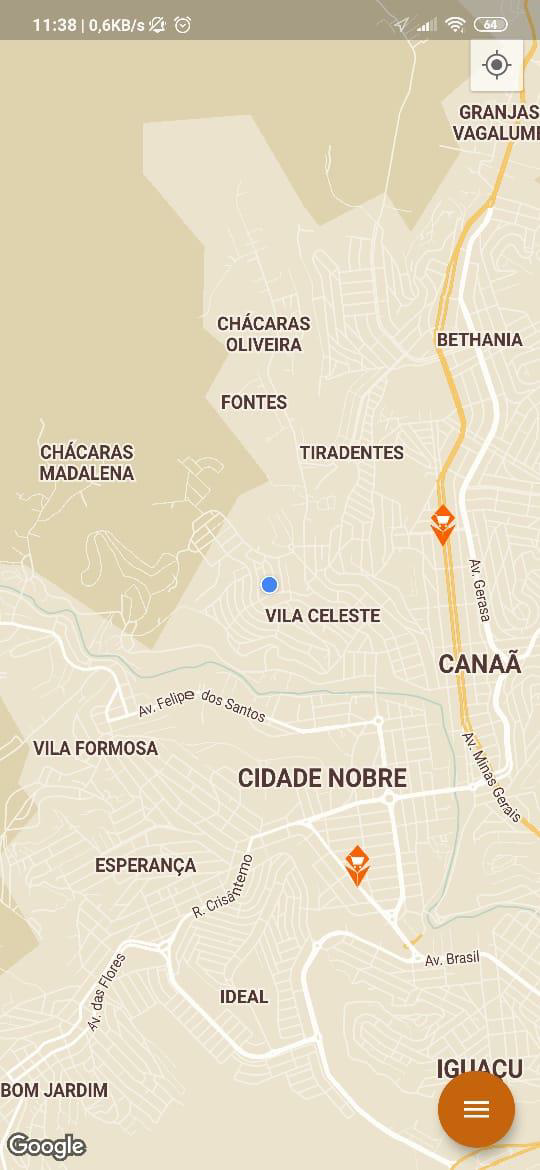
\includegraphics[scale=0.3]{Imagens/Print01.png}
    \fonte{Do autor - 2019.}
\end{figure}

Clicando no Menu no canto inferior direito, irá aparecer duas opções: “Produtos” e “Lista de Compras”.
\begin{figure}[H]
    \centering
    \caption{Tela Menu inferior.}
    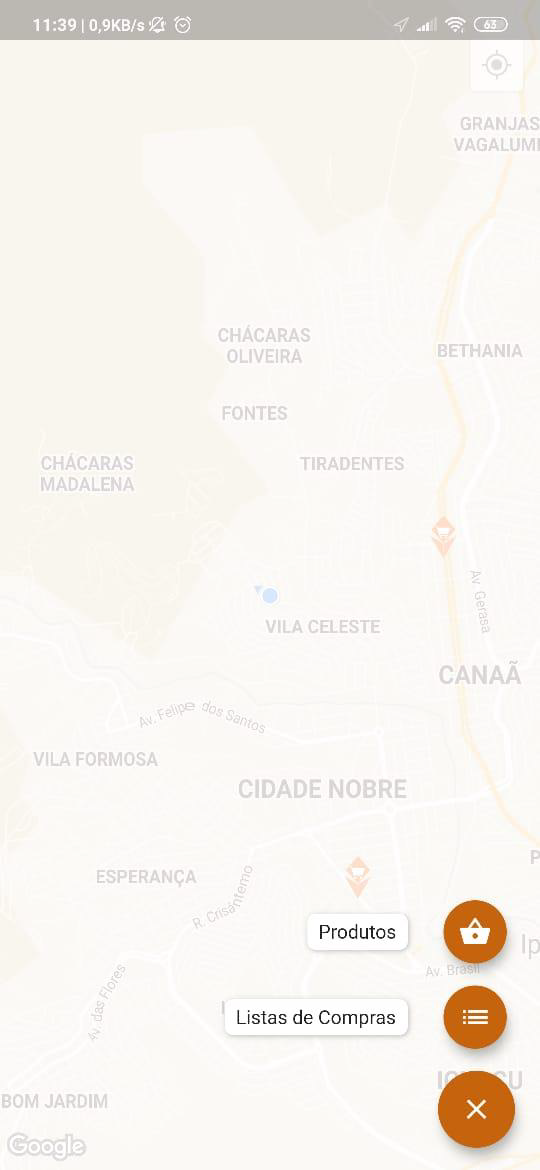
\includegraphics[scale=0.3]{Imagens/Print02.png}
    \fonte{Do autor - 2019.}
\end{figure}


Ao clicar em “Produtos” irá aparecer uma lista de todos os produtos cadastrados em nosso banco de dados. Arrastando o nome do produto para o lado direito aparecerá à imagem referente aquele produto em específico. Para retirar basta arrastar para o lado esquerdo.
\begin{figure}[H]
    \centering
    \caption{Tela Produtos.}
    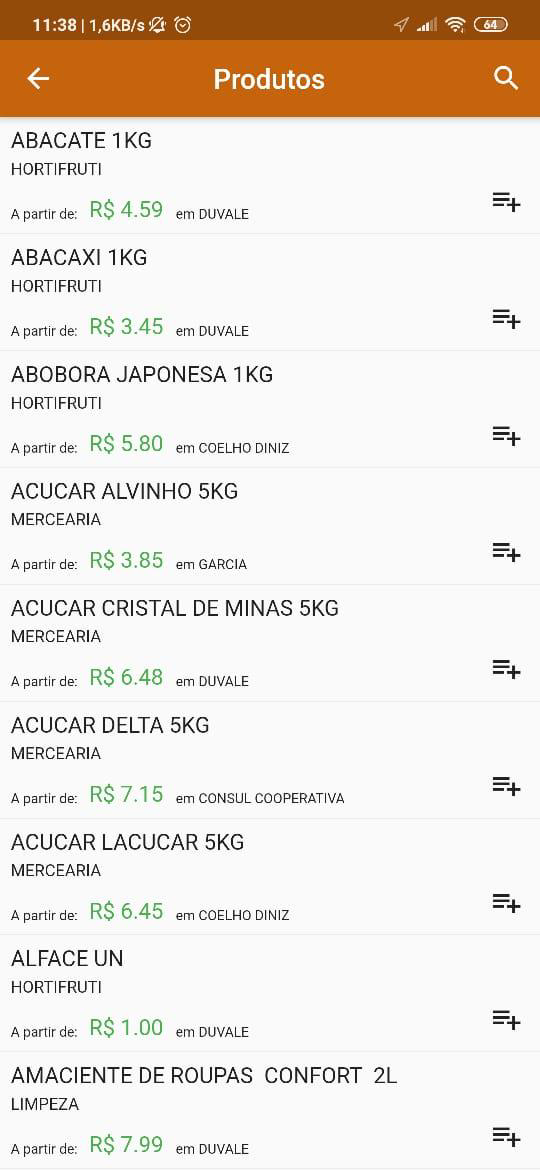
\includegraphics[scale=0.3]{Imagens/Print03.png}
    \fonte{Do autor - 2019.}
\end{figure}


Para adicionar um produto à lista basta clicar no símbolo à direita do mesmo, caso não tenha nenhuma lista cadastrada basta clicar em “Nova Lista”. Após nomear à lista basta confirmar e o item será adicionado.
\begin{figure}[H]
    \centering
    \caption{Tela Nova lista.}
    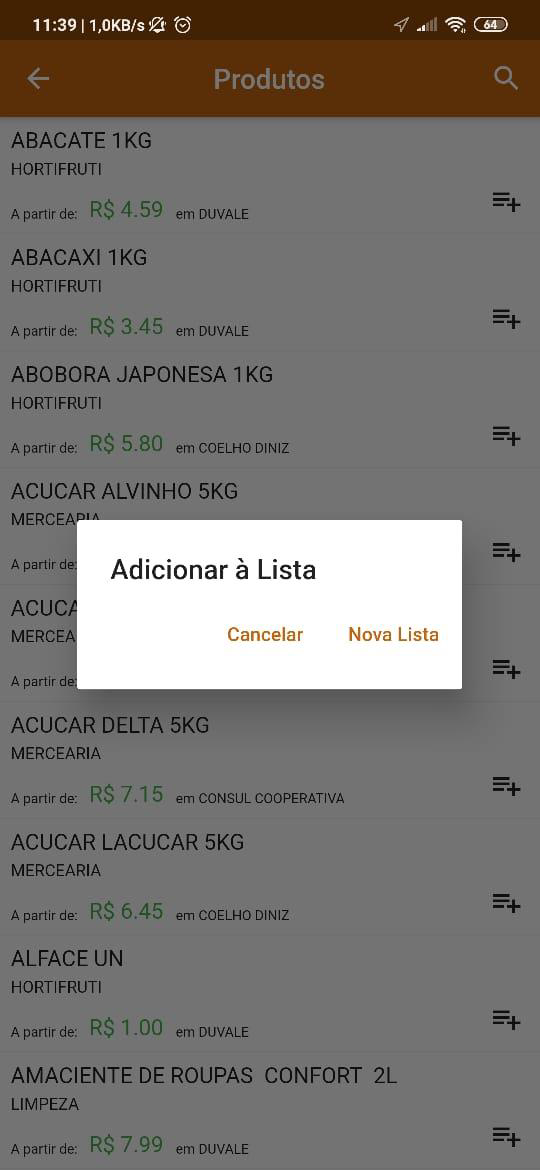
\includegraphics[scale=0.3]{Imagens/Print04.png}
    \fonte{Do autor - 2019.}
\end{figure}


Ao clicar em “Listas de Compras”, irão aparecer todas as listas já criadas com o número de produtos de cada lista.
\begin{figure}[H]
    \centering
    \caption{Tela Lista de compras.}
    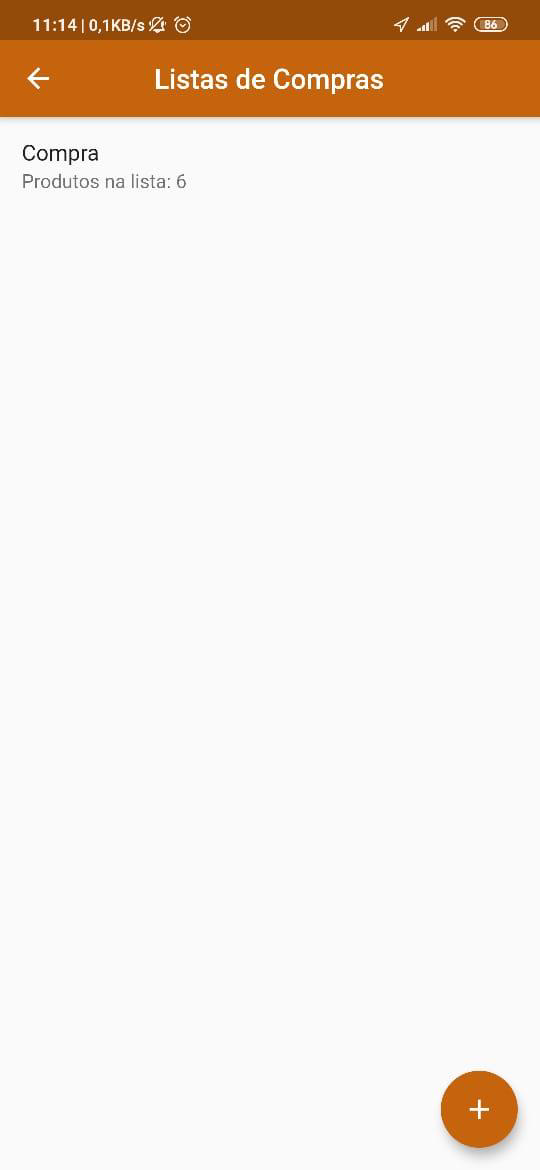
\includegraphics[scale=0.3]{Imagens/Print05.png}
    \fonte{Do autor - 2019.}
\end{figure}


Após selecionar uma lista vai aparecer um Menu com três opções: “Preços”, “Calcular Rota” e “Adicionar Produtos”. Ao selecionar “Preços” à aplicação retornará um ou dois valores. Se existir somente um valor significa que o local mais perto também é o mais barato, caso retorne dois valores, o da esquerda será o mais barato e o da direito o mais perto.
\begin{figure}[H]
    \centering
    \caption{Tela Menu de opções.}
    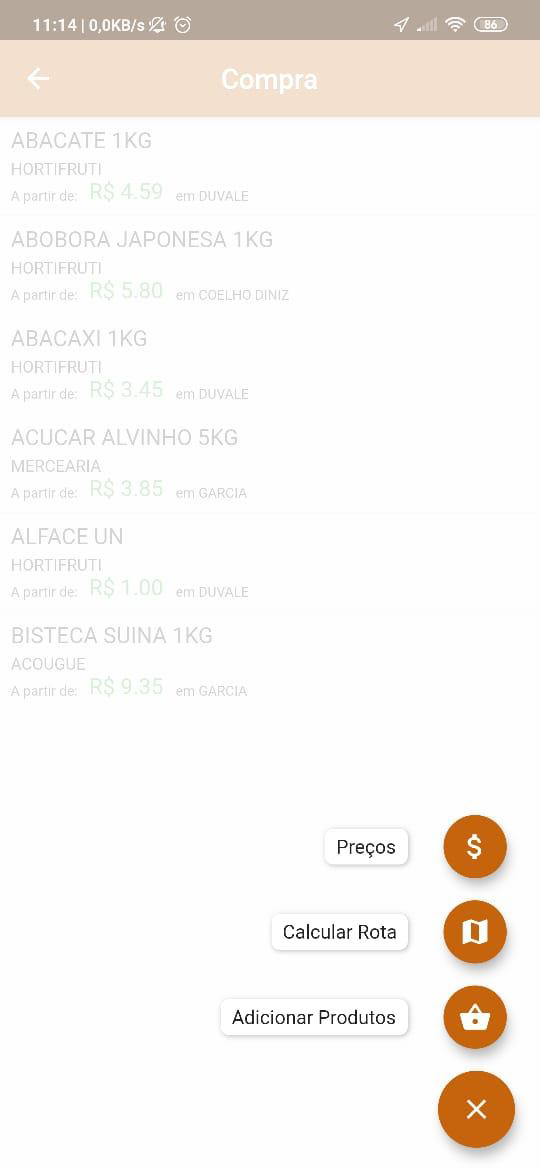
\includegraphics[scale=0.3]{Imagens/Print06.png}
    \fonte{Do autor - 2019.}
\end{figure}


Selecionando a opção “Rotas” o aplicativo estará mostrando a rota tanto do mais próximo quanto do mais barato. Ao clicar na opção desejada, a cor irá sobrepor a que não foi selecionada, podendo ser trocada em tempo de execução.
\begin{figure}[H]
    \centering
    \caption{Tela Rotas.}
    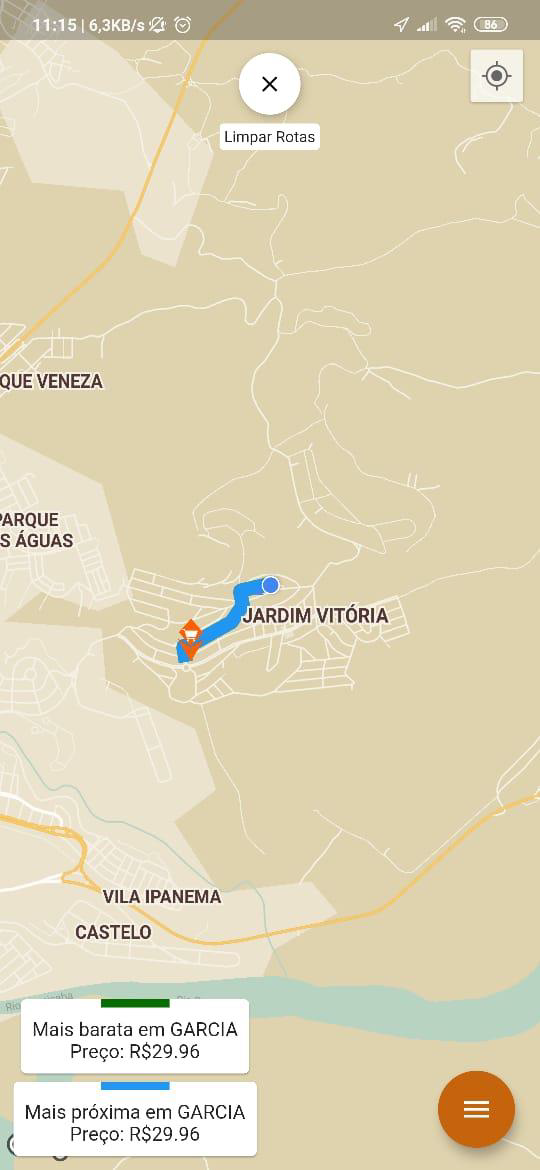
\includegraphics[scale=0.3]{Imagens/Print07.png}
    \fonte{Do autor - 2019.}
\end{figure}

%\chapter{Análise dos Dados}
%Digite seu texto nesse campo.

% ----------------------------------------------------------
% Finaliza a parte no bookmark do PDF
% para que se inicie o bookmark na raiz
% e adiciona espaço de parte no Sumário
% ----------------------------------------------------------
%\phantompart

%%%%%%%%%%%%%%%
%% Conclusão %%
%%%%%%%%%%%%%%%

%%%%%%%%%%%%%%%%%%%%%%%%%%%%%%%%%%%%%%%%%%%%%%%%%%%%%
%% Inserir seu texto da conclusão no campo abaixo %%
%%%%%%%%%%%%%%%%%%%%%%%%%%%%%%%%%%%%%%%%%%%%%%%%%%%%%
\chapter{Considerações Finais}

O presente trabalho cumpre ao requisito proposto, que é disponibilizar a seus usuários rotas otimizadas para realizar suas compras, sendo possível encontrar o menor preço do produto em si ou encontrar o estabelecimento mais próximo.
Desenvolver algoritmos para mapeamentos e cálculo de rotas seria bastante custoso, mas o uso da tecnologia Google Maps e suas ferramentas para este fim possibilitou tal função nesta aplicação. Possibilitando aos usuários realizarem uma lista de compras e instantaneamente descobrirem qual supermercado terá o menor valor, ou podendo levar em conta qual é o supermercado mais próximo de sua geolocalização que contém tais produtos.
De acordo com a pesquisa realizada com clientes (supostos usuários), o aplicativo seria viável e muito bem aceito por estes, pois atualmente as pessoas não dispõem de tanto tempo livre e não querem abrir mão de economizar. Na pesquisa anteriormente citada nota-se opiniões bem distintas quando se refere à aceitação do aplicativo pelos donos de comércio, pois alguns entrevistados opinaram que isso não seria tão viável para os estabelecimentos por questões de \textit{marketing}, entretanto não se pode esquecer que nos tempos atuais empresas inovadoras criam necessidades mesmo quando essas não existem, o que não é o caso desse aplicativo, já que supre uma necessidade existente. Outro ponto é o fato das empresas de sucesso, principalmente do ramo tecnológico, conquistarem os clientes para só depois conquistarem as organizações, ou seja, as empresas que querem se manter abertas se adaptam aos clientes e não o contrário.

%%%%%%%%%%%%%%%%%%%%%%%%%%%%
%% ELEMENTOS PÓS-TEXTUAIS %%
%%%%%%%%%%%%%%%%%%%%%%%%%%%%

%\postextual

%%%%%%%%%%%%%%%%%%%%%%%%%%%%%%%%
%% Referências bibliográficas %%
%%%%%%%%%%%%%%%%%%%%%%%%%%%%%%%%

\bibliography{Referencia}

%%%%%%%%%%%%%%%
%% Glossário %%
%%%%%%%%%%%%%%%

% Consulte o manual da classe abntex2 para orientações sobre o glossário.

%\glossary

%%%%%%%%%%%%%%%
%% Apêndices %%
%%%%%%%%%%%%%%%

%\begin{apendicesenv}
%\setlength{\parindent}{0pt}
% Imprime uma página indicando o início dos apêndices
%\partapendices*
%Digite seu texto nesse campo.

%\end{apendicesenv} 

%%%%%%%%%%%%
%% Anexos %%
%%%%%%%%%%%%

%\begin{anexosenv}

% Imprime uma página indicando o início dos anexos
\partanexos*

Digite seu texto nesse campo.

\end{anexosenv} 

%%%%%%%%%%%%%%%%%%%%%%
%% INDICE REMISSIVO %%
%%%%%%%%%%%%%%%%%%%%%%

\phantompart
\printindex

\end{document}